\documentclass[twoside]{book}

% Packages required by doxygen
\usepackage{fixltx2e}
\usepackage{calc}
\usepackage{doxygen}
\usepackage[export]{adjustbox} % also loads graphicx
\usepackage{graphicx}
\usepackage[utf8]{inputenc}
\usepackage{makeidx}
\usepackage{multicol}
\usepackage{multirow}
\PassOptionsToPackage{warn}{textcomp}
\usepackage{textcomp}
\usepackage[nointegrals]{wasysym}
\usepackage[table]{xcolor}

% Font selection
\usepackage[T1]{fontenc}
\usepackage[scaled=.90]{helvet}
\usepackage{courier}
\usepackage{amssymb}
\usepackage{sectsty}
\renewcommand{\familydefault}{\sfdefault}
\allsectionsfont{%
  \fontseries{bc}\selectfont%
  \color{darkgray}%
}
\renewcommand{\DoxyLabelFont}{%
  \fontseries{bc}\selectfont%
  \color{darkgray}%
}
\newcommand{\+}{\discretionary{\mbox{\scriptsize$\hookleftarrow$}}{}{}}

% Page & text layout
\usepackage{geometry}
\geometry{%
  a4paper,%
  top=2.5cm,%
  bottom=2.5cm,%
  left=2.5cm,%
  right=2.5cm%
}
\tolerance=750
\hfuzz=15pt
\hbadness=750
\setlength{\emergencystretch}{15pt}
\setlength{\parindent}{0cm}
\setlength{\parskip}{3ex plus 2ex minus 2ex}
\makeatletter
\renewcommand{\paragraph}{%
  \@startsection{paragraph}{4}{0ex}{-1.0ex}{1.0ex}{%
    \normalfont\normalsize\bfseries\SS@parafont%
  }%
}
\renewcommand{\subparagraph}{%
  \@startsection{subparagraph}{5}{0ex}{-1.0ex}{1.0ex}{%
    \normalfont\normalsize\bfseries\SS@subparafont%
  }%
}
\makeatother

% Headers & footers
\usepackage{fancyhdr}
\pagestyle{fancyplain}
\fancyhead[LE]{\fancyplain{}{\bfseries\thepage}}
\fancyhead[CE]{\fancyplain{}{}}
\fancyhead[RE]{\fancyplain{}{\bfseries\leftmark}}
\fancyhead[LO]{\fancyplain{}{\bfseries\rightmark}}
\fancyhead[CO]{\fancyplain{}{}}
\fancyhead[RO]{\fancyplain{}{\bfseries\thepage}}
\fancyfoot[LE]{\fancyplain{}{}}
\fancyfoot[CE]{\fancyplain{}{}}
\fancyfoot[RE]{\fancyplain{}{\bfseries\scriptsize Generated by Doxygen }}
\fancyfoot[LO]{\fancyplain{}{\bfseries\scriptsize Generated by Doxygen }}
\fancyfoot[CO]{\fancyplain{}{}}
\fancyfoot[RO]{\fancyplain{}{}}
\renewcommand{\footrulewidth}{0.4pt}
\renewcommand{\chaptermark}[1]{%
  \markboth{#1}{}%
}
\renewcommand{\sectionmark}[1]{%
  \markright{\thesection\ #1}%
}

% Indices & bibliography
\usepackage{natbib}
\usepackage[titles]{tocloft}
\setcounter{tocdepth}{3}
\setcounter{secnumdepth}{5}
\makeindex

% Hyperlinks (required, but should be loaded last)
\usepackage{ifpdf}
\ifpdf
  \usepackage[pdftex,pagebackref=true]{hyperref}
\else
  \usepackage[ps2pdf,pagebackref=true]{hyperref}
\fi
\hypersetup{%
  colorlinks=true,%
  linkcolor=blue,%
  citecolor=blue,%
  unicode%
}

% Custom commands
\newcommand{\clearemptydoublepage}{%
  \newpage{\pagestyle{empty}\cleardoublepage}%
}

\usepackage{caption}
\captionsetup{labelsep=space,justification=centering,font={bf},singlelinecheck=off,skip=4pt,position=top}

%===== C O N T E N T S =====

\begin{document}

% Titlepage & ToC
\hypersetup{pageanchor=false,
             bookmarksnumbered=true,
             pdfencoding=unicode
            }
\pagenumbering{alph}
\begin{titlepage}
\vspace*{7cm}
\begin{center}%
{\Large Projet Kyosai \\[1ex]\large 1.\+0 }\\
\vspace*{1cm}
{\large Generated by Doxygen 1.8.14}\\
\end{center}
\end{titlepage}
\clearemptydoublepage
\pagenumbering{roman}
\tableofcontents
\clearemptydoublepage
\pagenumbering{arabic}
\hypersetup{pageanchor=true}

%--- Begin generated contents ---
\chapter{Namespace Index}
\section{Namespace List}
Here is a list of all namespaces with brief descriptions\+:\begin{DoxyCompactList}
\item\contentsline{section}{\mbox{\hyperlink{namespace_app}{App}} }{\pageref{namespace_app}}{}
\item\contentsline{section}{\mbox{\hyperlink{namespace_app_1_1_controller}{App\textbackslash{}\+Controller}} }{\pageref{namespace_app_1_1_controller}}{}
\item\contentsline{section}{\mbox{\hyperlink{namespace_app_1_1_entity}{App\textbackslash{}\+Entity}} }{\pageref{namespace_app_1_1_entity}}{}
\item\contentsline{section}{\mbox{\hyperlink{namespace_app_1_1_repository}{App\textbackslash{}\+Repository}} }{\pageref{namespace_app_1_1_repository}}{}
\end{DoxyCompactList}

\chapter{Hierarchical Index}
\section{Class Hierarchy}
This inheritance list is sorted roughly, but not completely, alphabetically\+:\begin{DoxyCompactList}
\item Base\+Kernel\begin{DoxyCompactList}
\item \contentsline{section}{Kernel}{\pageref{class_app_1_1_kernel}}{}
\end{DoxyCompactList}
\item \contentsline{section}{Cart}{\pageref{class_app_1_1_entity_1_1_cart}}{}
\item \contentsline{section}{Category}{\pageref{class_app_1_1_entity_1_1_category}}{}
\item \contentsline{section}{Commande}{\pageref{class_app_1_1_entity_1_1_commande}}{}
\item \contentsline{section}{Produits}{\pageref{class_app_1_1_entity_1_1_produits}}{}
\item \contentsline{section}{Role}{\pageref{class_app_1_1_entity_1_1_role}}{}
\item Abstract\+Controller\begin{DoxyCompactList}
\item \contentsline{section}{Admin\+Edit\+Post\+Controller}{\pageref{class_app_1_1_controller_1_1_admin_edit_post_controller}}{}
\item \contentsline{section}{Api\+Shop\+Controller}{\pageref{class_app_1_1_controller_1_1_api_shop_controller}}{}
\item \contentsline{section}{Cart\+Controller}{\pageref{class_app_1_1_controller_1_1_cart_controller}}{}
\item \contentsline{section}{Mail\+Contact\+Controller}{\pageref{class_app_1_1_controller_1_1_mail_contact_controller}}{}
\item \contentsline{section}{User\+Controller}{\pageref{class_app_1_1_controller_1_1_user_controller}}{}
\end{DoxyCompactList}
\item Service\+Entity\+Repository\begin{DoxyCompactList}
\item \contentsline{section}{Cart\+Repository}{\pageref{class_app_1_1_repository_1_1_cart_repository}}{}
\item \contentsline{section}{Category\+Repository}{\pageref{class_app_1_1_repository_1_1_category_repository}}{}
\item \contentsline{section}{Commande\+Repository}{\pageref{class_app_1_1_repository_1_1_commande_repository}}{}
\item \contentsline{section}{Produits\+Repository}{\pageref{class_app_1_1_repository_1_1_produits_repository}}{}
\item \contentsline{section}{Role\+Repository}{\pageref{class_app_1_1_repository_1_1_role_repository}}{}
\item \contentsline{section}{Users\+Repository}{\pageref{class_app_1_1_repository_1_1_users_repository}}{}
\end{DoxyCompactList}
\item User\+Interface\begin{DoxyCompactList}
\item \contentsline{section}{Users}{\pageref{class_app_1_1_entity_1_1_users}}{}
\end{DoxyCompactList}
\end{DoxyCompactList}

\chapter{Data Structure Index}
\section{Data Structures}
Here are the data structures with brief descriptions\+:\begin{DoxyCompactList}
\item\contentsline{section}{\mbox{\hyperlink{class_app_1_1_controller_1_1_admin_edit_post_controller}{Admin\+Edit\+Post\+Controller}} }{\pageref{class_app_1_1_controller_1_1_admin_edit_post_controller}}{}
\item\contentsline{section}{\mbox{\hyperlink{class_app_1_1_controller_1_1_api_shop_controller}{Api\+Shop\+Controller}} }{\pageref{class_app_1_1_controller_1_1_api_shop_controller}}{}
\item\contentsline{section}{\mbox{\hyperlink{class_app_1_1_entity_1_1_cart}{Cart}} }{\pageref{class_app_1_1_entity_1_1_cart}}{}
\item\contentsline{section}{\mbox{\hyperlink{class_app_1_1_controller_1_1_cart_controller}{Cart\+Controller}} }{\pageref{class_app_1_1_controller_1_1_cart_controller}}{}
\item\contentsline{section}{\mbox{\hyperlink{class_app_1_1_repository_1_1_cart_repository}{Cart\+Repository}} }{\pageref{class_app_1_1_repository_1_1_cart_repository}}{}
\item\contentsline{section}{\mbox{\hyperlink{class_app_1_1_entity_1_1_category}{Category}} }{\pageref{class_app_1_1_entity_1_1_category}}{}
\item\contentsline{section}{\mbox{\hyperlink{class_app_1_1_repository_1_1_category_repository}{Category\+Repository}} }{\pageref{class_app_1_1_repository_1_1_category_repository}}{}
\item\contentsline{section}{\mbox{\hyperlink{class_app_1_1_entity_1_1_commande}{Commande}} }{\pageref{class_app_1_1_entity_1_1_commande}}{}
\item\contentsline{section}{\mbox{\hyperlink{class_app_1_1_repository_1_1_commande_repository}{Commande\+Repository}} }{\pageref{class_app_1_1_repository_1_1_commande_repository}}{}
\item\contentsline{section}{\mbox{\hyperlink{class_app_1_1_kernel}{Kernel}} }{\pageref{class_app_1_1_kernel}}{}
\item\contentsline{section}{\mbox{\hyperlink{class_app_1_1_controller_1_1_mail_contact_controller}{Mail\+Contact\+Controller}} }{\pageref{class_app_1_1_controller_1_1_mail_contact_controller}}{}
\item\contentsline{section}{\mbox{\hyperlink{class_app_1_1_entity_1_1_produits}{Produits}} }{\pageref{class_app_1_1_entity_1_1_produits}}{}
\item\contentsline{section}{\mbox{\hyperlink{class_app_1_1_repository_1_1_produits_repository}{Produits\+Repository}} }{\pageref{class_app_1_1_repository_1_1_produits_repository}}{}
\item\contentsline{section}{\mbox{\hyperlink{class_app_1_1_entity_1_1_role}{Role}} }{\pageref{class_app_1_1_entity_1_1_role}}{}
\item\contentsline{section}{\mbox{\hyperlink{class_app_1_1_repository_1_1_role_repository}{Role\+Repository}} }{\pageref{class_app_1_1_repository_1_1_role_repository}}{}
\item\contentsline{section}{\mbox{\hyperlink{class_app_1_1_controller_1_1_user_controller}{User\+Controller}} }{\pageref{class_app_1_1_controller_1_1_user_controller}}{}
\item\contentsline{section}{\mbox{\hyperlink{class_app_1_1_entity_1_1_users}{Users}} }{\pageref{class_app_1_1_entity_1_1_users}}{}
\item\contentsline{section}{\mbox{\hyperlink{class_app_1_1_repository_1_1_users_repository}{Users\+Repository}} }{\pageref{class_app_1_1_repository_1_1_users_repository}}{}
\end{DoxyCompactList}

\chapter{File Index}
\section{File List}
Here is a list of all files with brief descriptions\+:\begin{DoxyCompactList}
\item\contentsline{section}{src/\mbox{\hyperlink{_kernel_8php}{Kernel.\+php}} }{\pageref{_kernel_8php}}{}
\item\contentsline{section}{src/\+Controller/\mbox{\hyperlink{_admin_edit_post_controller_8php}{Admin\+Edit\+Post\+Controller.\+php}} }{\pageref{_admin_edit_post_controller_8php}}{}
\item\contentsline{section}{src/\+Controller/\mbox{\hyperlink{_api_shop_controller_8php}{Api\+Shop\+Controller.\+php}} }{\pageref{_api_shop_controller_8php}}{}
\item\contentsline{section}{src/\+Controller/\mbox{\hyperlink{_cart_controller_8php}{Cart\+Controller.\+php}} }{\pageref{_cart_controller_8php}}{}
\item\contentsline{section}{src/\+Controller/\mbox{\hyperlink{_mail_contact_controller_8php}{Mail\+Contact\+Controller.\+php}} }{\pageref{_mail_contact_controller_8php}}{}
\item\contentsline{section}{src/\+Controller/\mbox{\hyperlink{_user_controller_8php}{User\+Controller.\+php}} }{\pageref{_user_controller_8php}}{}
\item\contentsline{section}{src/\+Entity/\mbox{\hyperlink{_cart_8php}{Cart.\+php}} }{\pageref{_cart_8php}}{}
\item\contentsline{section}{src/\+Entity/\mbox{\hyperlink{_category_8php}{Category.\+php}} }{\pageref{_category_8php}}{}
\item\contentsline{section}{src/\+Entity/\mbox{\hyperlink{_commande_8php}{Commande.\+php}} }{\pageref{_commande_8php}}{}
\item\contentsline{section}{src/\+Entity/\mbox{\hyperlink{_produits_8php}{Produits.\+php}} }{\pageref{_produits_8php}}{}
\item\contentsline{section}{src/\+Entity/\mbox{\hyperlink{_role_8php}{Role.\+php}} }{\pageref{_role_8php}}{}
\item\contentsline{section}{src/\+Entity/\mbox{\hyperlink{_users_8php}{Users.\+php}} }{\pageref{_users_8php}}{}
\item\contentsline{section}{src/\+Repository/\mbox{\hyperlink{_cart_repository_8php}{Cart\+Repository.\+php}} }{\pageref{_cart_repository_8php}}{}
\item\contentsline{section}{src/\+Repository/\mbox{\hyperlink{_category_repository_8php}{Category\+Repository.\+php}} }{\pageref{_category_repository_8php}}{}
\item\contentsline{section}{src/\+Repository/\mbox{\hyperlink{_commande_repository_8php}{Commande\+Repository.\+php}} }{\pageref{_commande_repository_8php}}{}
\item\contentsline{section}{src/\+Repository/\mbox{\hyperlink{_produits_repository_8php}{Produits\+Repository.\+php}} }{\pageref{_produits_repository_8php}}{}
\item\contentsline{section}{src/\+Repository/\mbox{\hyperlink{_role_repository_8php}{Role\+Repository.\+php}} }{\pageref{_role_repository_8php}}{}
\item\contentsline{section}{src/\+Repository/\mbox{\hyperlink{_users_repository_8php}{Users\+Repository.\+php}} }{\pageref{_users_repository_8php}}{}
\end{DoxyCompactList}

\chapter{Namespace Documentation}
\hypertarget{namespace_app}{}\section{App Namespace Reference}
\label{namespace_app}\index{App@{App}}
\subsection*{Namespaces}
\begin{DoxyCompactItemize}
\item 
 \mbox{\hyperlink{namespace_app_1_1_controller}{Controller}}
\item 
 \mbox{\hyperlink{namespace_app_1_1_entity}{Entity}}
\item 
 \mbox{\hyperlink{namespace_app_1_1_repository}{Repository}}
\end{DoxyCompactItemize}
\subsection*{Data Structures}
\begin{DoxyCompactItemize}
\item 
class \mbox{\hyperlink{class_app_1_1_kernel}{Kernel}}
\end{DoxyCompactItemize}

\hypertarget{namespace_app_1_1_controller}{}\section{App\textbackslash{}Controller Namespace Reference}
\label{namespace_app_1_1_controller}\index{App\textbackslash{}\+Controller@{App\textbackslash{}\+Controller}}
\subsection*{Data Structures}
\begin{DoxyCompactItemize}
\item 
class \mbox{\hyperlink{class_app_1_1_controller_1_1_admin_edit_post_controller}{Admin\+Edit\+Post\+Controller}}
\item 
class \mbox{\hyperlink{class_app_1_1_controller_1_1_api_shop_controller}{Api\+Shop\+Controller}}
\item 
class \mbox{\hyperlink{class_app_1_1_controller_1_1_cart_controller}{Cart\+Controller}}
\item 
class \mbox{\hyperlink{class_app_1_1_controller_1_1_mail_contact_controller}{Mail\+Contact\+Controller}}
\item 
class \mbox{\hyperlink{class_app_1_1_controller_1_1_user_controller}{User\+Controller}}
\end{DoxyCompactItemize}

\hypertarget{namespace_app_1_1_entity}{}\section{App\textbackslash{}Entity Namespace Reference}
\label{namespace_app_1_1_entity}\index{App\textbackslash{}\+Entity@{App\textbackslash{}\+Entity}}
\subsection*{Data Structures}
\begin{DoxyCompactItemize}
\item 
class \mbox{\hyperlink{class_app_1_1_entity_1_1_cart}{Cart}}
\item 
class \mbox{\hyperlink{class_app_1_1_entity_1_1_category}{Category}}
\item 
class \mbox{\hyperlink{class_app_1_1_entity_1_1_commande}{Commande}}
\item 
class \mbox{\hyperlink{class_app_1_1_entity_1_1_produits}{Produits}}
\item 
class \mbox{\hyperlink{class_app_1_1_entity_1_1_role}{Role}}
\item 
class \mbox{\hyperlink{class_app_1_1_entity_1_1_users}{Users}}
\end{DoxyCompactItemize}

\hypertarget{namespace_app_1_1_repository}{}\section{App\textbackslash{}Repository Namespace Reference}
\label{namespace_app_1_1_repository}\index{App\textbackslash{}\+Repository@{App\textbackslash{}\+Repository}}
\subsection*{Data Structures}
\begin{DoxyCompactItemize}
\item 
class \mbox{\hyperlink{class_app_1_1_repository_1_1_cart_repository}{Cart\+Repository}}
\item 
class \mbox{\hyperlink{class_app_1_1_repository_1_1_category_repository}{Category\+Repository}}
\item 
class \mbox{\hyperlink{class_app_1_1_repository_1_1_commande_repository}{Commande\+Repository}}
\item 
class \mbox{\hyperlink{class_app_1_1_repository_1_1_produits_repository}{Produits\+Repository}}
\item 
class \mbox{\hyperlink{class_app_1_1_repository_1_1_role_repository}{Role\+Repository}}
\item 
class \mbox{\hyperlink{class_app_1_1_repository_1_1_users_repository}{Users\+Repository}}
\end{DoxyCompactItemize}

\chapter{Data Structure Documentation}
\hypertarget{class_app_1_1_controller_1_1_admin_edit_post_controller}{}\section{Admin\+Edit\+Post\+Controller Class Reference}
\label{class_app_1_1_controller_1_1_admin_edit_post_controller}\index{Admin\+Edit\+Post\+Controller@{Admin\+Edit\+Post\+Controller}}
Inheritance diagram for Admin\+Edit\+Post\+Controller\+:\begin{figure}[H]
\begin{center}
\leavevmode
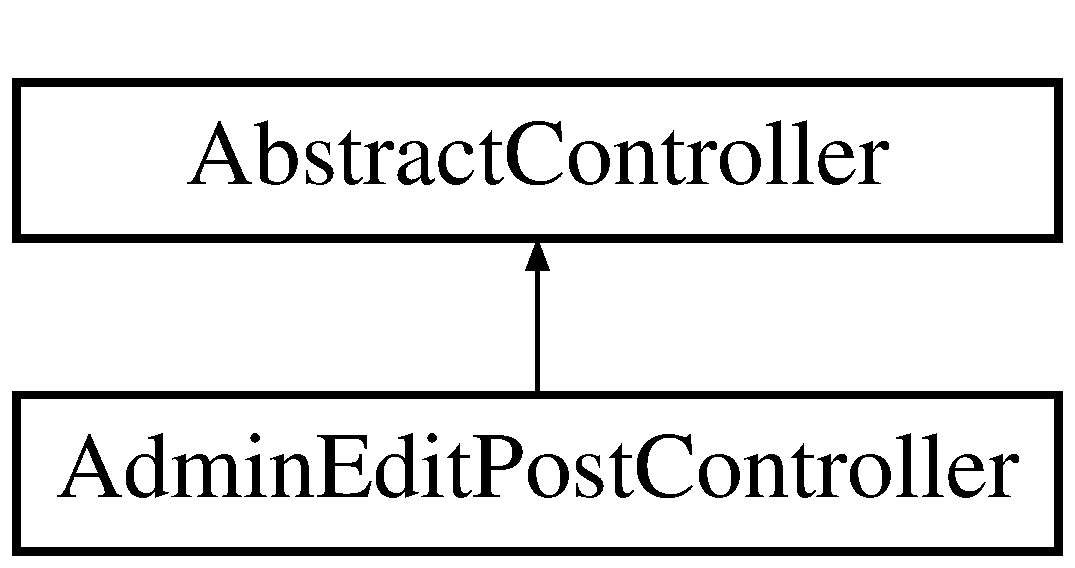
\includegraphics[height=2.000000cm]{class_app_1_1_controller_1_1_admin_edit_post_controller}
\end{center}
\end{figure}
\subsection*{Public Member Functions}
\begin{DoxyCompactItemize}
\item 
\mbox{\hyperlink{class_app_1_1_controller_1_1_admin_edit_post_controller_a125dd362544d79e6056e4b57cb43135b}{index}} (Request \$request, Entity\+Manager\+Interface \$manager, \mbox{\hyperlink{class_app_1_1_repository_1_1_category_repository}{Category\+Repository}} \$category\+Repository)
\item 
\mbox{\hyperlink{class_app_1_1_controller_1_1_admin_edit_post_controller_ab65e87c7f80014f2b687f789eba6d3b4}{get\+Edit\+Content}} (int \$id, \mbox{\hyperlink{class_app_1_1_repository_1_1_produits_repository}{Produits\+Repository}} \$produit)
\item 
\mbox{\hyperlink{class_app_1_1_controller_1_1_admin_edit_post_controller_a0578b6f3be8a0c7857aa19c7e343db4c}{edit}} (int \$id, \mbox{\hyperlink{class_app_1_1_repository_1_1_produits_repository}{Produits\+Repository}} \$produit\+Repository, Request \$request, Entity\+Manager\+Interface \$manager, \mbox{\hyperlink{class_app_1_1_repository_1_1_category_repository}{Category\+Repository}} \$category\+Repository)
\item 
\mbox{\hyperlink{class_app_1_1_controller_1_1_admin_edit_post_controller_af982d7c8be1c44eb293d63ab7920592b}{delete}} (int \$id, \mbox{\hyperlink{class_app_1_1_repository_1_1_produits_repository}{Produits\+Repository}} \$produit, Entity\+Manager\+Interface \$manager)
\end{DoxyCompactItemize}


\subsection{Detailed Description}
Manages the operations to be performed on a product from the administration page \begin{DoxyAuthor}{Author}
Michael B\+E\+C\+Q\+U\+ER 
\end{DoxyAuthor}


\subsection{Member Function Documentation}
\mbox{\Hypertarget{class_app_1_1_controller_1_1_admin_edit_post_controller_af982d7c8be1c44eb293d63ab7920592b}\label{class_app_1_1_controller_1_1_admin_edit_post_controller_af982d7c8be1c44eb293d63ab7920592b}} 
\index{App\+::\+Controller\+::\+Admin\+Edit\+Post\+Controller@{App\+::\+Controller\+::\+Admin\+Edit\+Post\+Controller}!delete@{delete}}
\index{delete@{delete}!App\+::\+Controller\+::\+Admin\+Edit\+Post\+Controller@{App\+::\+Controller\+::\+Admin\+Edit\+Post\+Controller}}
\subsubsection{\texorpdfstring{delete()}{delete()}}
{\footnotesize\ttfamily delete (\begin{DoxyParamCaption}\item[{int}]{\$id,  }\item[{\mbox{\hyperlink{class_app_1_1_repository_1_1_produits_repository}{Produits\+Repository}}}]{\$produit,  }\item[{Entity\+Manager\+Interface}]{\$manager }\end{DoxyParamCaption})}

(\char`\"{}/api/admin/delete/\{id\}\char`\"{}, name=\char`\"{}api\+\_\+admin\+\_\+delete\char`\"{}, methods=\{\char`\"{}\+G\+E\+T\char`\"{}\} ) Delete the product


\begin{DoxyParams}[1]{Parameters}
mixed & {\em \$id} & \\
\hline
mixed & {\em \$produit} & \\
\hline
mixed & {\em \$manager} & \\
\hline
\end{DoxyParams}
\begin{DoxyReturn}{Returns}
void 
\end{DoxyReturn}
\mbox{\Hypertarget{class_app_1_1_controller_1_1_admin_edit_post_controller_a0578b6f3be8a0c7857aa19c7e343db4c}\label{class_app_1_1_controller_1_1_admin_edit_post_controller_a0578b6f3be8a0c7857aa19c7e343db4c}} 
\index{App\+::\+Controller\+::\+Admin\+Edit\+Post\+Controller@{App\+::\+Controller\+::\+Admin\+Edit\+Post\+Controller}!edit@{edit}}
\index{edit@{edit}!App\+::\+Controller\+::\+Admin\+Edit\+Post\+Controller@{App\+::\+Controller\+::\+Admin\+Edit\+Post\+Controller}}
\subsubsection{\texorpdfstring{edit()}{edit()}}
{\footnotesize\ttfamily edit (\begin{DoxyParamCaption}\item[{int}]{\$id,  }\item[{\mbox{\hyperlink{class_app_1_1_repository_1_1_produits_repository}{Produits\+Repository}}}]{\$produit\+Repository,  }\item[{Request}]{\$request,  }\item[{Entity\+Manager\+Interface}]{\$manager,  }\item[{\mbox{\hyperlink{class_app_1_1_repository_1_1_category_repository}{Category\+Repository}}}]{\$category\+Repository }\end{DoxyParamCaption})}

(\char`\"{}/api/admin/edit/\{id\}\char`\"{}, name=\char`\"{}api\+\_\+admin\+\_\+edit\char`\"{}, methods=\{\char`\"{}\+P\+O\+S\+T\char`\"{}\}) Modify the product


\begin{DoxyParams}[1]{Parameters}
integer & {\em \$id} & \\
\hline
mixed & {\em \$produit\+Repository} & \\
\hline
mixed & {\em \$request} & \\
\hline
mixed & {\em \$manager} & \\
\hline
mixed & {\em \$category\+Repository} & \\
\hline
\end{DoxyParams}
\begin{DoxyReturn}{Returns}
void 
\end{DoxyReturn}
\mbox{\Hypertarget{class_app_1_1_controller_1_1_admin_edit_post_controller_ab65e87c7f80014f2b687f789eba6d3b4}\label{class_app_1_1_controller_1_1_admin_edit_post_controller_ab65e87c7f80014f2b687f789eba6d3b4}} 
\index{App\+::\+Controller\+::\+Admin\+Edit\+Post\+Controller@{App\+::\+Controller\+::\+Admin\+Edit\+Post\+Controller}!get\+Edit\+Content@{get\+Edit\+Content}}
\index{get\+Edit\+Content@{get\+Edit\+Content}!App\+::\+Controller\+::\+Admin\+Edit\+Post\+Controller@{App\+::\+Controller\+::\+Admin\+Edit\+Post\+Controller}}
\subsubsection{\texorpdfstring{get\+Edit\+Content()}{getEditContent()}}
{\footnotesize\ttfamily get\+Edit\+Content (\begin{DoxyParamCaption}\item[{int}]{\$id,  }\item[{\mbox{\hyperlink{class_app_1_1_repository_1_1_produits_repository}{Produits\+Repository}}}]{\$produit }\end{DoxyParamCaption})}

(\char`\"{}/api/admin/edit/view/\{id\}\char`\"{}, name=\char`\"{}api\+\_\+admin\+\_\+edit\+\_\+view\char`\"{}, methods=\{\char`\"{}\+G\+E\+T\char`\"{}\}) Display the product


\begin{DoxyParams}[1]{Parameters}
integer & {\em \$id} & \\
\hline
mixed & {\em \$produit} & \\
\hline
\end{DoxyParams}
\begin{DoxyReturn}{Returns}
void 
\end{DoxyReturn}
\mbox{\Hypertarget{class_app_1_1_controller_1_1_admin_edit_post_controller_a125dd362544d79e6056e4b57cb43135b}\label{class_app_1_1_controller_1_1_admin_edit_post_controller_a125dd362544d79e6056e4b57cb43135b}} 
\index{App\+::\+Controller\+::\+Admin\+Edit\+Post\+Controller@{App\+::\+Controller\+::\+Admin\+Edit\+Post\+Controller}!index@{index}}
\index{index@{index}!App\+::\+Controller\+::\+Admin\+Edit\+Post\+Controller@{App\+::\+Controller\+::\+Admin\+Edit\+Post\+Controller}}
\subsubsection{\texorpdfstring{index()}{index()}}
{\footnotesize\ttfamily index (\begin{DoxyParamCaption}\item[{Request}]{\$request,  }\item[{Entity\+Manager\+Interface}]{\$manager,  }\item[{\mbox{\hyperlink{class_app_1_1_repository_1_1_category_repository}{Category\+Repository}}}]{\$category\+Repository }\end{DoxyParamCaption})}

(\char`\"{}/api/admin\char`\"{}, name=\char`\"{}api\+\_\+admin\+\_\+index\char`\"{}, methods=\{\char`\"{}\+P\+O\+S\+T\char`\"{}\}) Add a product to the administration page


\begin{DoxyParams}[1]{Parameters}
mixed & {\em \$request} & \\
\hline
mixed & {\em \$manager} & \\
\hline
mixed & {\em \$category\+Repository} & \\
\hline
\end{DoxyParams}
\begin{DoxyReturn}{Returns}
Response 
\end{DoxyReturn}


The documentation for this class was generated from the following file\+:\begin{DoxyCompactItemize}
\item 
src/\+Controller/\mbox{\hyperlink{_admin_edit_post_controller_8php}{Admin\+Edit\+Post\+Controller.\+php}}\end{DoxyCompactItemize}

\hypertarget{class_app_1_1_controller_1_1_api_shop_controller}{}\section{Api\+Shop\+Controller Class Reference}
\label{class_app_1_1_controller_1_1_api_shop_controller}\index{Api\+Shop\+Controller@{Api\+Shop\+Controller}}
Inheritance diagram for Api\+Shop\+Controller\+:\begin{figure}[H]
\begin{center}
\leavevmode
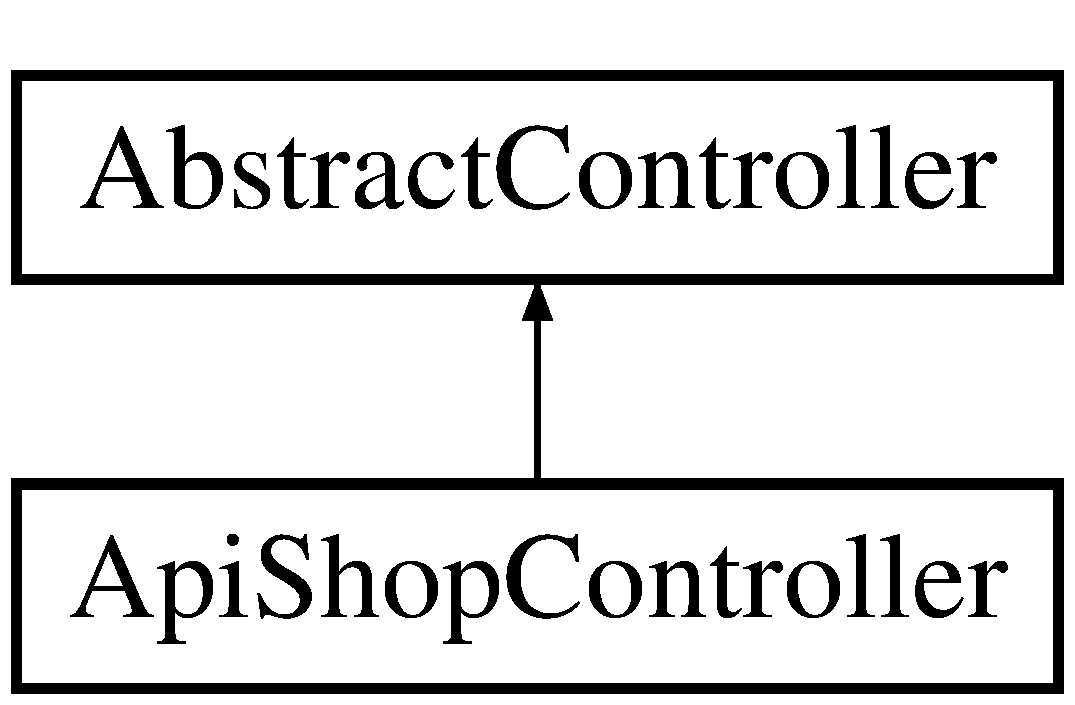
\includegraphics[height=2.000000cm]{class_app_1_1_controller_1_1_api_shop_controller}
\end{center}
\end{figure}
\subsection*{Public Member Functions}
\begin{DoxyCompactItemize}
\item 
\mbox{\hyperlink{class_app_1_1_controller_1_1_api_shop_controller_a4b18c8720ede9d5ce2beda028d675d13}{index}} (\mbox{\hyperlink{class_app_1_1_repository_1_1_produits_repository}{Produits\+Repository}} \$produits\+Repository)
\item 
\mbox{\hyperlink{class_app_1_1_controller_1_1_api_shop_controller_aa17be29d9a8068e407db7d0db06bde6d}{category\+List}} (\mbox{\hyperlink{class_app_1_1_repository_1_1_category_repository}{Category\+Repository}} \$category\+Repository)
\end{DoxyCompactItemize}


\subsection{Detailed Description}
Retrieves the various product information from the database \begin{DoxyAuthor}{Author}
Michael B\+E\+C\+Q\+U\+ER 
\end{DoxyAuthor}


\subsection{Member Function Documentation}
\mbox{\Hypertarget{class_app_1_1_controller_1_1_api_shop_controller_aa17be29d9a8068e407db7d0db06bde6d}\label{class_app_1_1_controller_1_1_api_shop_controller_aa17be29d9a8068e407db7d0db06bde6d}} 
\index{App\+::\+Controller\+::\+Api\+Shop\+Controller@{App\+::\+Controller\+::\+Api\+Shop\+Controller}!category\+List@{category\+List}}
\index{category\+List@{category\+List}!App\+::\+Controller\+::\+Api\+Shop\+Controller@{App\+::\+Controller\+::\+Api\+Shop\+Controller}}
\subsubsection{\texorpdfstring{category\+List()}{categoryList()}}
{\footnotesize\ttfamily category\+List (\begin{DoxyParamCaption}\item[{\mbox{\hyperlink{class_app_1_1_repository_1_1_category_repository}{Category\+Repository}}}]{\$category\+Repository }\end{DoxyParamCaption})}

(\char`\"{}/category/list\char`\"{}, name=\char`\"{}category\+\_\+list\char`\"{}, methods=\{\char`\"{}\+G\+E\+T\char`\"{}\}) Retrieves the list of product categories


\begin{DoxyParams}[1]{Parameters}
mixed & {\em \$category\+Repository} & \\
\hline
\end{DoxyParams}
\begin{DoxyReturn}{Returns}
response 
\end{DoxyReturn}
\mbox{\Hypertarget{class_app_1_1_controller_1_1_api_shop_controller_a4b18c8720ede9d5ce2beda028d675d13}\label{class_app_1_1_controller_1_1_api_shop_controller_a4b18c8720ede9d5ce2beda028d675d13}} 
\index{App\+::\+Controller\+::\+Api\+Shop\+Controller@{App\+::\+Controller\+::\+Api\+Shop\+Controller}!index@{index}}
\index{index@{index}!App\+::\+Controller\+::\+Api\+Shop\+Controller@{App\+::\+Controller\+::\+Api\+Shop\+Controller}}
\subsubsection{\texorpdfstring{index()}{index()}}
{\footnotesize\ttfamily index (\begin{DoxyParamCaption}\item[{\mbox{\hyperlink{class_app_1_1_repository_1_1_produits_repository}{Produits\+Repository}}}]{\$produits\+Repository }\end{DoxyParamCaption})}

(\char`\"{}/shop\char`\"{}, name=\char`\"{}shop\+\_\+index\char`\"{}, methods=\{\char`\"{}\+G\+E\+T\char`\"{}\}) Retrieves products from the database


\begin{DoxyParams}[1]{Parameters}
mixed & {\em \$produits\+Repository} & \\
\hline
\end{DoxyParams}
\begin{DoxyReturn}{Returns}
response 
\end{DoxyReturn}


The documentation for this class was generated from the following file\+:\begin{DoxyCompactItemize}
\item 
src/\+Controller/\mbox{\hyperlink{_api_shop_controller_8php}{Api\+Shop\+Controller.\+php}}\end{DoxyCompactItemize}

\hypertarget{class_app_1_1_entity_1_1_cart}{}\section{Cart Class Reference}
\label{class_app_1_1_entity_1_1_cart}\index{Cart@{Cart}}
\subsection*{Public Member Functions}
\begin{DoxyCompactItemize}
\item 
\mbox{\hyperlink{class_app_1_1_entity_1_1_cart_a12251d0c022e9e21c137a105ff683f13}{get\+Id}} ()
\item 
\mbox{\hyperlink{class_app_1_1_entity_1_1_cart_abae8ce0df3d9f49efcba4904a2d030a6}{get\+Quantity}} ()
\item 
\mbox{\hyperlink{class_app_1_1_entity_1_1_cart_a6aaf2dab8685fde29dbdf49b782017df}{set\+Quantity}} (int \$quantity)
\item 
\mbox{\hyperlink{class_app_1_1_entity_1_1_cart_ae81b7186fb97a7c6457edcc68c9aa2ef}{get\+User}} ()
\item 
\mbox{\hyperlink{class_app_1_1_entity_1_1_cart_a31170564fe4585dda0eb916f17323681}{set\+User}} (?\mbox{\hyperlink{class_app_1_1_entity_1_1_users}{Users}} \$user)
\item 
\mbox{\hyperlink{class_app_1_1_entity_1_1_cart_aa39b956895038a1e65f2a0ca81fd3398}{get\+Produit}} ()
\item 
\mbox{\hyperlink{class_app_1_1_entity_1_1_cart_aee1aa682ba8a05574c94b12e4a4bbc73}{set\+Produit}} (?\mbox{\hyperlink{class_app_1_1_entity_1_1_produits}{Produits}} \$produit)
\end{DoxyCompactItemize}


\subsection{Detailed Description}
() (repository\+Class=Cart\+Repository\+::class) 

\subsection{Member Function Documentation}
\mbox{\Hypertarget{class_app_1_1_entity_1_1_cart_a12251d0c022e9e21c137a105ff683f13}\label{class_app_1_1_entity_1_1_cart_a12251d0c022e9e21c137a105ff683f13}} 
\index{App\+::\+Entity\+::\+Cart@{App\+::\+Entity\+::\+Cart}!get\+Id@{get\+Id}}
\index{get\+Id@{get\+Id}!App\+::\+Entity\+::\+Cart@{App\+::\+Entity\+::\+Cart}}
\subsubsection{\texorpdfstring{get\+Id()}{getId()}}
{\footnotesize\ttfamily get\+Id (\begin{DoxyParamCaption}{ }\end{DoxyParamCaption})}

\mbox{\Hypertarget{class_app_1_1_entity_1_1_cart_aa39b956895038a1e65f2a0ca81fd3398}\label{class_app_1_1_entity_1_1_cart_aa39b956895038a1e65f2a0ca81fd3398}} 
\index{App\+::\+Entity\+::\+Cart@{App\+::\+Entity\+::\+Cart}!get\+Produit@{get\+Produit}}
\index{get\+Produit@{get\+Produit}!App\+::\+Entity\+::\+Cart@{App\+::\+Entity\+::\+Cart}}
\subsubsection{\texorpdfstring{get\+Produit()}{getProduit()}}
{\footnotesize\ttfamily get\+Produit (\begin{DoxyParamCaption}{ }\end{DoxyParamCaption})}

\mbox{\Hypertarget{class_app_1_1_entity_1_1_cart_abae8ce0df3d9f49efcba4904a2d030a6}\label{class_app_1_1_entity_1_1_cart_abae8ce0df3d9f49efcba4904a2d030a6}} 
\index{App\+::\+Entity\+::\+Cart@{App\+::\+Entity\+::\+Cart}!get\+Quantity@{get\+Quantity}}
\index{get\+Quantity@{get\+Quantity}!App\+::\+Entity\+::\+Cart@{App\+::\+Entity\+::\+Cart}}
\subsubsection{\texorpdfstring{get\+Quantity()}{getQuantity()}}
{\footnotesize\ttfamily get\+Quantity (\begin{DoxyParamCaption}{ }\end{DoxyParamCaption})}

\mbox{\Hypertarget{class_app_1_1_entity_1_1_cart_ae81b7186fb97a7c6457edcc68c9aa2ef}\label{class_app_1_1_entity_1_1_cart_ae81b7186fb97a7c6457edcc68c9aa2ef}} 
\index{App\+::\+Entity\+::\+Cart@{App\+::\+Entity\+::\+Cart}!get\+User@{get\+User}}
\index{get\+User@{get\+User}!App\+::\+Entity\+::\+Cart@{App\+::\+Entity\+::\+Cart}}
\subsubsection{\texorpdfstring{get\+User()}{getUser()}}
{\footnotesize\ttfamily get\+User (\begin{DoxyParamCaption}{ }\end{DoxyParamCaption})}

\mbox{\Hypertarget{class_app_1_1_entity_1_1_cart_aee1aa682ba8a05574c94b12e4a4bbc73}\label{class_app_1_1_entity_1_1_cart_aee1aa682ba8a05574c94b12e4a4bbc73}} 
\index{App\+::\+Entity\+::\+Cart@{App\+::\+Entity\+::\+Cart}!set\+Produit@{set\+Produit}}
\index{set\+Produit@{set\+Produit}!App\+::\+Entity\+::\+Cart@{App\+::\+Entity\+::\+Cart}}
\subsubsection{\texorpdfstring{set\+Produit()}{setProduit()}}
{\footnotesize\ttfamily set\+Produit (\begin{DoxyParamCaption}\item[{?\mbox{\hyperlink{class_app_1_1_entity_1_1_produits}{Produits}}}]{\$produit }\end{DoxyParamCaption})}

\mbox{\Hypertarget{class_app_1_1_entity_1_1_cart_a6aaf2dab8685fde29dbdf49b782017df}\label{class_app_1_1_entity_1_1_cart_a6aaf2dab8685fde29dbdf49b782017df}} 
\index{App\+::\+Entity\+::\+Cart@{App\+::\+Entity\+::\+Cart}!set\+Quantity@{set\+Quantity}}
\index{set\+Quantity@{set\+Quantity}!App\+::\+Entity\+::\+Cart@{App\+::\+Entity\+::\+Cart}}
\subsubsection{\texorpdfstring{set\+Quantity()}{setQuantity()}}
{\footnotesize\ttfamily set\+Quantity (\begin{DoxyParamCaption}\item[{int}]{\$quantity }\end{DoxyParamCaption})}

\mbox{\Hypertarget{class_app_1_1_entity_1_1_cart_a31170564fe4585dda0eb916f17323681}\label{class_app_1_1_entity_1_1_cart_a31170564fe4585dda0eb916f17323681}} 
\index{App\+::\+Entity\+::\+Cart@{App\+::\+Entity\+::\+Cart}!set\+User@{set\+User}}
\index{set\+User@{set\+User}!App\+::\+Entity\+::\+Cart@{App\+::\+Entity\+::\+Cart}}
\subsubsection{\texorpdfstring{set\+User()}{setUser()}}
{\footnotesize\ttfamily set\+User (\begin{DoxyParamCaption}\item[{?\mbox{\hyperlink{class_app_1_1_entity_1_1_users}{Users}}}]{\$user }\end{DoxyParamCaption})}



The documentation for this class was generated from the following file\+:\begin{DoxyCompactItemize}
\item 
src/\+Entity/\mbox{\hyperlink{_cart_8php}{Cart.\+php}}\end{DoxyCompactItemize}

\hypertarget{class_app_1_1_controller_1_1_cart_controller}{}\section{Cart\+Controller Class Reference}
\label{class_app_1_1_controller_1_1_cart_controller}\index{Cart\+Controller@{Cart\+Controller}}
Inheritance diagram for Cart\+Controller\+:\begin{figure}[H]
\begin{center}
\leavevmode
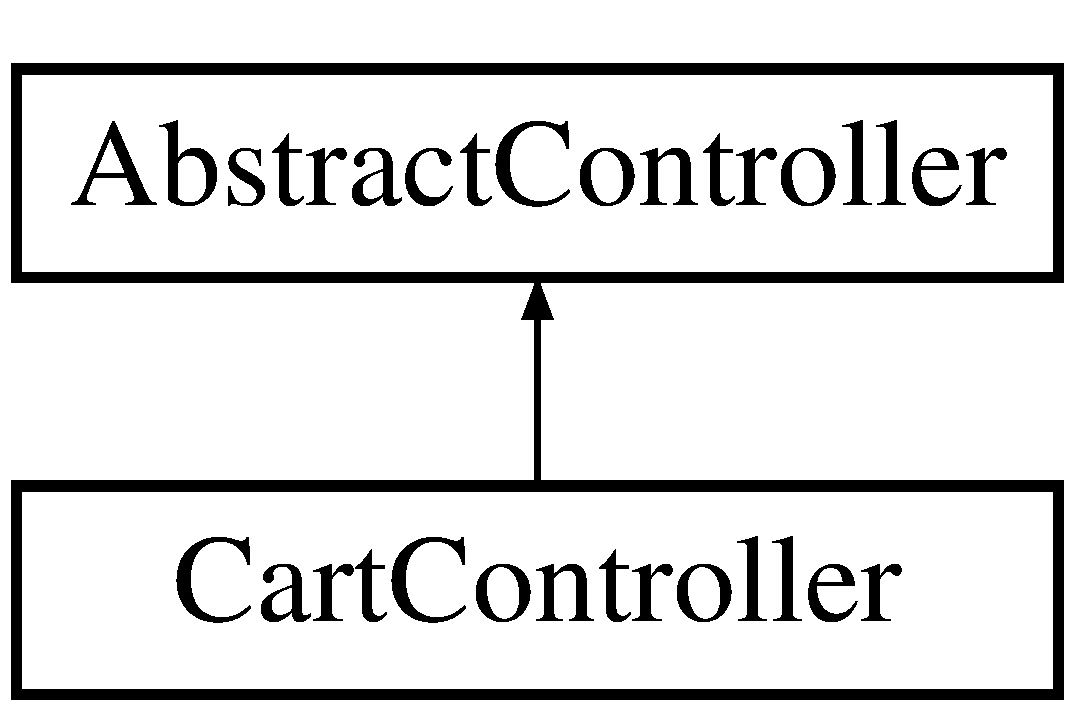
\includegraphics[height=2.000000cm]{class_app_1_1_controller_1_1_cart_controller}
\end{center}
\end{figure}
\subsection*{Public Member Functions}
\begin{DoxyCompactItemize}
\item 
\mbox{\hyperlink{class_app_1_1_controller_1_1_cart_controller_acb4819cf06207b3c628edfa1a5af6a6f}{index}} (\mbox{\hyperlink{class_app_1_1_repository_1_1_users_repository}{Users\+Repository}} \$user\+Repository, Request \$request)
\item 
\mbox{\hyperlink{class_app_1_1_controller_1_1_cart_controller_ac217678855013811414d24f84ad9b57b}{add}} (Request \$request, \mbox{\hyperlink{class_app_1_1_repository_1_1_users_repository}{Users\+Repository}} \$user\+Repository, \mbox{\hyperlink{class_app_1_1_repository_1_1_produits_repository}{Produits\+Repository}} \$produits\+Repository, Entity\+Manager\+Interface \$manager, \mbox{\hyperlink{class_app_1_1_entity_1_1_produits}{Produits}} \$produit\+Entity, \mbox{\hyperlink{class_app_1_1_repository_1_1_cart_repository}{Cart\+Repository}} \$cart\+Repository)
\item 
\mbox{\hyperlink{class_app_1_1_controller_1_1_cart_controller_a0a4f4fa16921c0100dcd9d64104eafdb}{delete}} (int \$id, Entity\+Manager\+Interface \$manager, \mbox{\hyperlink{class_app_1_1_repository_1_1_cart_repository}{Cart\+Repository}} \$cart\+Repository)
\end{DoxyCompactItemize}


\subsection{Detailed Description}
Manages the various cart operations \begin{DoxyAuthor}{Author}
Michael B\+E\+C\+Q\+U\+ER 
\end{DoxyAuthor}


\subsection{Member Function Documentation}
\mbox{\Hypertarget{class_app_1_1_controller_1_1_cart_controller_ac217678855013811414d24f84ad9b57b}\label{class_app_1_1_controller_1_1_cart_controller_ac217678855013811414d24f84ad9b57b}} 
\index{App\+::\+Controller\+::\+Cart\+Controller@{App\+::\+Controller\+::\+Cart\+Controller}!add@{add}}
\index{add@{add}!App\+::\+Controller\+::\+Cart\+Controller@{App\+::\+Controller\+::\+Cart\+Controller}}
\subsubsection{\texorpdfstring{add()}{add()}}
{\footnotesize\ttfamily add (\begin{DoxyParamCaption}\item[{Request}]{\$request,  }\item[{\mbox{\hyperlink{class_app_1_1_repository_1_1_users_repository}{Users\+Repository}}}]{\$user\+Repository,  }\item[{\mbox{\hyperlink{class_app_1_1_repository_1_1_produits_repository}{Produits\+Repository}}}]{\$produits\+Repository,  }\item[{Entity\+Manager\+Interface}]{\$manager,  }\item[{\mbox{\hyperlink{class_app_1_1_entity_1_1_produits}{Produits}}}]{\$produit\+Entity,  }\item[{\mbox{\hyperlink{class_app_1_1_repository_1_1_cart_repository}{Cart\+Repository}}}]{\$cart\+Repository }\end{DoxyParamCaption})}

(\char`\"{}/add/cart/\{id\}\char`\"{}, name=\char`\"{}add\+\_\+cart\char`\"{}, methods=\{\char`\"{}\+G\+E\+T\char`\"{}\}) Add a product to the user\textquotesingle{}s cart


\begin{DoxyParams}[1]{Parameters}
mixed & {\em \$request} & \\
\hline
mixed & {\em \$user\+Repository} & \\
\hline
mixed & {\em \$produits\+Repository} & \\
\hline
mixed & {\em \$manager} & \\
\hline
mixed & {\em \$produit\+Entity} & \\
\hline
mixed & {\em \$cart\+Repository} & \\
\hline
\end{DoxyParams}
\begin{DoxyReturn}{Returns}
void 
\end{DoxyReturn}
\mbox{\Hypertarget{class_app_1_1_controller_1_1_cart_controller_a0a4f4fa16921c0100dcd9d64104eafdb}\label{class_app_1_1_controller_1_1_cart_controller_a0a4f4fa16921c0100dcd9d64104eafdb}} 
\index{App\+::\+Controller\+::\+Cart\+Controller@{App\+::\+Controller\+::\+Cart\+Controller}!delete@{delete}}
\index{delete@{delete}!App\+::\+Controller\+::\+Cart\+Controller@{App\+::\+Controller\+::\+Cart\+Controller}}
\subsubsection{\texorpdfstring{delete()}{delete()}}
{\footnotesize\ttfamily delete (\begin{DoxyParamCaption}\item[{int}]{\$id,  }\item[{Entity\+Manager\+Interface}]{\$manager,  }\item[{\mbox{\hyperlink{class_app_1_1_repository_1_1_cart_repository}{Cart\+Repository}}}]{\$cart\+Repository }\end{DoxyParamCaption})}

(\char`\"{}/delete/cart/\{id\}\char`\"{}, name=\char`\"{}delete\+\_\+cart\char`\"{}, methods=\{\char`\"{}\+D\+E\+L\+E\+T\+E\char`\"{}\}) Delete a product from the user\textquotesingle{}s cart


\begin{DoxyParams}[1]{Parameters}
integer & {\em \$id} & \\
\hline
mixed & {\em \$manager} & \\
\hline
mixed & {\em \$cart\+Repository} & \\
\hline
\end{DoxyParams}
\begin{DoxyReturn}{Returns}
void 
\end{DoxyReturn}
\mbox{\Hypertarget{class_app_1_1_controller_1_1_cart_controller_acb4819cf06207b3c628edfa1a5af6a6f}\label{class_app_1_1_controller_1_1_cart_controller_acb4819cf06207b3c628edfa1a5af6a6f}} 
\index{App\+::\+Controller\+::\+Cart\+Controller@{App\+::\+Controller\+::\+Cart\+Controller}!index@{index}}
\index{index@{index}!App\+::\+Controller\+::\+Cart\+Controller@{App\+::\+Controller\+::\+Cart\+Controller}}
\subsubsection{\texorpdfstring{index()}{index()}}
{\footnotesize\ttfamily index (\begin{DoxyParamCaption}\item[{\mbox{\hyperlink{class_app_1_1_repository_1_1_users_repository}{Users\+Repository}}}]{\$user\+Repository,  }\item[{Request}]{\$request }\end{DoxyParamCaption})}

(\char`\"{}/panier\char`\"{}, name=\char`\"{}cart\+\_\+index\char`\"{}, methods=\{\char`\"{}\+G\+E\+T\char`\"{}\}) Retrieves the user\textquotesingle{}s cart


\begin{DoxyParams}[1]{Parameters}
mixed & {\em \$user\+Repository} & \\
\hline
mixed & {\em \$request} & \\
\hline
\end{DoxyParams}
\begin{DoxyReturn}{Returns}
void 
\end{DoxyReturn}


The documentation for this class was generated from the following file\+:\begin{DoxyCompactItemize}
\item 
src/\+Controller/\mbox{\hyperlink{_cart_controller_8php}{Cart\+Controller.\+php}}\end{DoxyCompactItemize}

\hypertarget{class_app_1_1_repository_1_1_cart_repository}{}\section{Cart\+Repository Class Reference}
\label{class_app_1_1_repository_1_1_cart_repository}\index{Cart\+Repository@{Cart\+Repository}}
Inheritance diagram for Cart\+Repository\+:\begin{figure}[H]
\begin{center}
\leavevmode
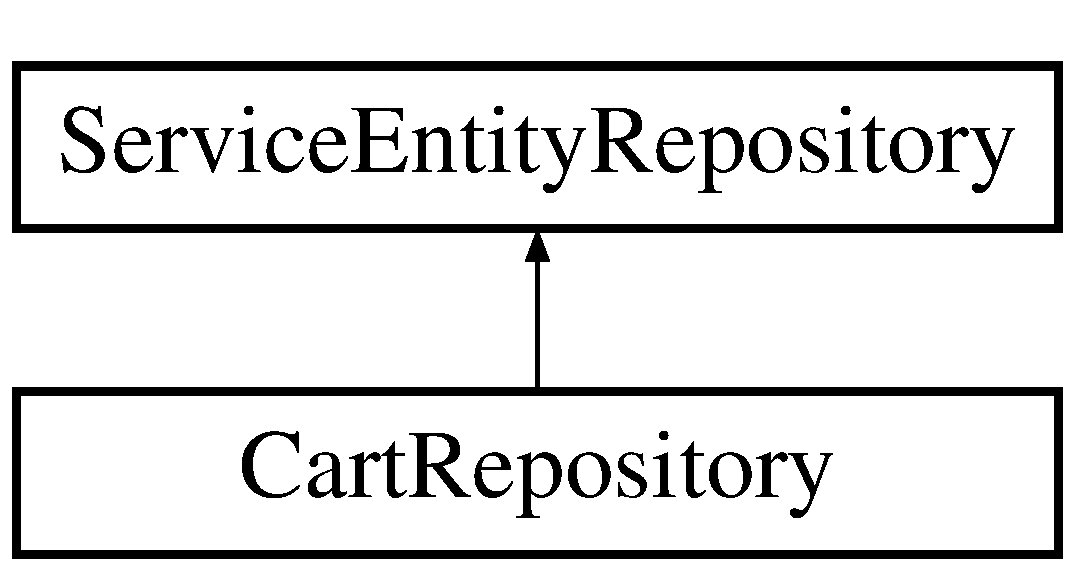
\includegraphics[height=2.000000cm]{class_app_1_1_repository_1_1_cart_repository}
\end{center}
\end{figure}
\subsection*{Public Member Functions}
\begin{DoxyCompactItemize}
\item 
\mbox{\hyperlink{class_app_1_1_repository_1_1_cart_repository_a38ea33dde11163765f358f5f10a3bc03}{\+\_\+\+\_\+construct}} (Manager\+Registry \$registry)
\end{DoxyCompactItemize}


\subsection{Detailed Description}
Cart$\vert$null find(\$id, \$lock\+Mode = null, \$lock\+Version = null)  Cart$\vert$null find\+One\+By(array \$criteria, array \$order\+By = null)  Cart\mbox{[}\mbox{]} find\+All()  Cart\mbox{[}\mbox{]} find\+By(array \$criteria, array \$order\+By = null, \$limit = null, \$offset = null) 

\subsection{Constructor \& Destructor Documentation}
\mbox{\Hypertarget{class_app_1_1_repository_1_1_cart_repository_a38ea33dde11163765f358f5f10a3bc03}\label{class_app_1_1_repository_1_1_cart_repository_a38ea33dde11163765f358f5f10a3bc03}} 
\index{App\+::\+Repository\+::\+Cart\+Repository@{App\+::\+Repository\+::\+Cart\+Repository}!\+\_\+\+\_\+construct@{\+\_\+\+\_\+construct}}
\index{\+\_\+\+\_\+construct@{\+\_\+\+\_\+construct}!App\+::\+Repository\+::\+Cart\+Repository@{App\+::\+Repository\+::\+Cart\+Repository}}
\subsubsection{\texorpdfstring{\+\_\+\+\_\+construct()}{\_\_construct()}}
{\footnotesize\ttfamily \+\_\+\+\_\+construct (\begin{DoxyParamCaption}\item[{Manager\+Registry}]{\$registry }\end{DoxyParamCaption})}



The documentation for this class was generated from the following file\+:\begin{DoxyCompactItemize}
\item 
src/\+Repository/\mbox{\hyperlink{_cart_repository_8php}{Cart\+Repository.\+php}}\end{DoxyCompactItemize}

\hypertarget{class_app_1_1_entity_1_1_category}{}\section{Category Class Reference}
\label{class_app_1_1_entity_1_1_category}\index{Category@{Category}}
\subsection*{Public Member Functions}
\begin{DoxyCompactItemize}
\item 
\mbox{\hyperlink{class_app_1_1_entity_1_1_category_a095c5d389db211932136b53f25f39685}{\+\_\+\+\_\+construct}} ()
\item 
\mbox{\hyperlink{class_app_1_1_entity_1_1_category_a12251d0c022e9e21c137a105ff683f13}{get\+Id}} ()
\item 
\mbox{\hyperlink{class_app_1_1_entity_1_1_category_a14c4e7420d903d3e40342266333d2ecf}{get\+Label}} ()
\item 
\mbox{\hyperlink{class_app_1_1_entity_1_1_category_adc435edb6ffd860b94dc2561a6cdb2be}{set\+Label}} (string \$label)
\item 
\mbox{\hyperlink{class_app_1_1_entity_1_1_category_ac4ae2b107901ad7dd44af9821aba87c7}{get\+Produits}} ()
\item 
\mbox{\hyperlink{class_app_1_1_entity_1_1_category_a5875f1e30c617aab128df24fd45d22b1}{add\+Produit}} (\mbox{\hyperlink{class_app_1_1_entity_1_1_produits}{Produits}} \$produit)
\item 
\mbox{\hyperlink{class_app_1_1_entity_1_1_category_a737ead4d9c5fb03ce667d58783ce74c9}{remove\+Produit}} (\mbox{\hyperlink{class_app_1_1_entity_1_1_produits}{Produits}} \$produit)
\end{DoxyCompactItemize}


\subsection{Detailed Description}
() (repository\+Class=Category\+Repository\+::class) 

\subsection{Constructor \& Destructor Documentation}
\mbox{\Hypertarget{class_app_1_1_entity_1_1_category_a095c5d389db211932136b53f25f39685}\label{class_app_1_1_entity_1_1_category_a095c5d389db211932136b53f25f39685}} 
\index{App\+::\+Entity\+::\+Category@{App\+::\+Entity\+::\+Category}!\+\_\+\+\_\+construct@{\+\_\+\+\_\+construct}}
\index{\+\_\+\+\_\+construct@{\+\_\+\+\_\+construct}!App\+::\+Entity\+::\+Category@{App\+::\+Entity\+::\+Category}}
\subsubsection{\texorpdfstring{\+\_\+\+\_\+construct()}{\_\_construct()}}
{\footnotesize\ttfamily \+\_\+\+\_\+construct (\begin{DoxyParamCaption}{ }\end{DoxyParamCaption})}



\subsection{Member Function Documentation}
\mbox{\Hypertarget{class_app_1_1_entity_1_1_category_a5875f1e30c617aab128df24fd45d22b1}\label{class_app_1_1_entity_1_1_category_a5875f1e30c617aab128df24fd45d22b1}} 
\index{App\+::\+Entity\+::\+Category@{App\+::\+Entity\+::\+Category}!add\+Produit@{add\+Produit}}
\index{add\+Produit@{add\+Produit}!App\+::\+Entity\+::\+Category@{App\+::\+Entity\+::\+Category}}
\subsubsection{\texorpdfstring{add\+Produit()}{addProduit()}}
{\footnotesize\ttfamily add\+Produit (\begin{DoxyParamCaption}\item[{\mbox{\hyperlink{class_app_1_1_entity_1_1_produits}{Produits}}}]{\$produit }\end{DoxyParamCaption})}

\mbox{\Hypertarget{class_app_1_1_entity_1_1_category_a12251d0c022e9e21c137a105ff683f13}\label{class_app_1_1_entity_1_1_category_a12251d0c022e9e21c137a105ff683f13}} 
\index{App\+::\+Entity\+::\+Category@{App\+::\+Entity\+::\+Category}!get\+Id@{get\+Id}}
\index{get\+Id@{get\+Id}!App\+::\+Entity\+::\+Category@{App\+::\+Entity\+::\+Category}}
\subsubsection{\texorpdfstring{get\+Id()}{getId()}}
{\footnotesize\ttfamily get\+Id (\begin{DoxyParamCaption}{ }\end{DoxyParamCaption})}

\mbox{\Hypertarget{class_app_1_1_entity_1_1_category_a14c4e7420d903d3e40342266333d2ecf}\label{class_app_1_1_entity_1_1_category_a14c4e7420d903d3e40342266333d2ecf}} 
\index{App\+::\+Entity\+::\+Category@{App\+::\+Entity\+::\+Category}!get\+Label@{get\+Label}}
\index{get\+Label@{get\+Label}!App\+::\+Entity\+::\+Category@{App\+::\+Entity\+::\+Category}}
\subsubsection{\texorpdfstring{get\+Label()}{getLabel()}}
{\footnotesize\ttfamily get\+Label (\begin{DoxyParamCaption}{ }\end{DoxyParamCaption})}

\mbox{\Hypertarget{class_app_1_1_entity_1_1_category_ac4ae2b107901ad7dd44af9821aba87c7}\label{class_app_1_1_entity_1_1_category_ac4ae2b107901ad7dd44af9821aba87c7}} 
\index{App\+::\+Entity\+::\+Category@{App\+::\+Entity\+::\+Category}!get\+Produits@{get\+Produits}}
\index{get\+Produits@{get\+Produits}!App\+::\+Entity\+::\+Category@{App\+::\+Entity\+::\+Category}}
\subsubsection{\texorpdfstring{get\+Produits()}{getProduits()}}
{\footnotesize\ttfamily get\+Produits (\begin{DoxyParamCaption}{ }\end{DoxyParamCaption})}

\begin{DoxyReturn}{Returns}
Collection$\vert$\+Produits\mbox{[}\mbox{]} 
\end{DoxyReturn}
\mbox{\Hypertarget{class_app_1_1_entity_1_1_category_a737ead4d9c5fb03ce667d58783ce74c9}\label{class_app_1_1_entity_1_1_category_a737ead4d9c5fb03ce667d58783ce74c9}} 
\index{App\+::\+Entity\+::\+Category@{App\+::\+Entity\+::\+Category}!remove\+Produit@{remove\+Produit}}
\index{remove\+Produit@{remove\+Produit}!App\+::\+Entity\+::\+Category@{App\+::\+Entity\+::\+Category}}
\subsubsection{\texorpdfstring{remove\+Produit()}{removeProduit()}}
{\footnotesize\ttfamily remove\+Produit (\begin{DoxyParamCaption}\item[{\mbox{\hyperlink{class_app_1_1_entity_1_1_produits}{Produits}}}]{\$produit }\end{DoxyParamCaption})}

\mbox{\Hypertarget{class_app_1_1_entity_1_1_category_adc435edb6ffd860b94dc2561a6cdb2be}\label{class_app_1_1_entity_1_1_category_adc435edb6ffd860b94dc2561a6cdb2be}} 
\index{App\+::\+Entity\+::\+Category@{App\+::\+Entity\+::\+Category}!set\+Label@{set\+Label}}
\index{set\+Label@{set\+Label}!App\+::\+Entity\+::\+Category@{App\+::\+Entity\+::\+Category}}
\subsubsection{\texorpdfstring{set\+Label()}{setLabel()}}
{\footnotesize\ttfamily set\+Label (\begin{DoxyParamCaption}\item[{string}]{\$label }\end{DoxyParamCaption})}



The documentation for this class was generated from the following file\+:\begin{DoxyCompactItemize}
\item 
src/\+Entity/\mbox{\hyperlink{_category_8php}{Category.\+php}}\end{DoxyCompactItemize}

\hypertarget{class_app_1_1_repository_1_1_category_repository}{}\section{Category\+Repository Class Reference}
\label{class_app_1_1_repository_1_1_category_repository}\index{Category\+Repository@{Category\+Repository}}
Inheritance diagram for Category\+Repository\+:\begin{figure}[H]
\begin{center}
\leavevmode
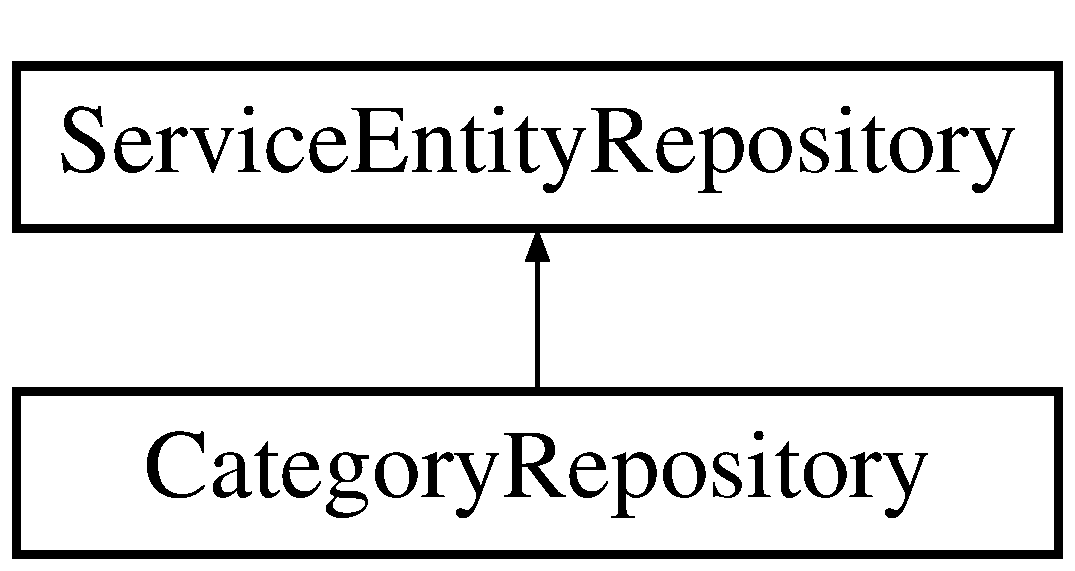
\includegraphics[height=2.000000cm]{class_app_1_1_repository_1_1_category_repository}
\end{center}
\end{figure}
\subsection*{Public Member Functions}
\begin{DoxyCompactItemize}
\item 
\mbox{\hyperlink{class_app_1_1_repository_1_1_category_repository_a38ea33dde11163765f358f5f10a3bc03}{\+\_\+\+\_\+construct}} (Manager\+Registry \$registry)
\end{DoxyCompactItemize}


\subsection{Detailed Description}
Category$\vert$null find(\$id, \$lock\+Mode = null, \$lock\+Version = null)  Category$\vert$null find\+One\+By(array \$criteria, array \$order\+By = null)  Category\mbox{[}\mbox{]} find\+All()  Category\mbox{[}\mbox{]} find\+By(array \$criteria, array \$order\+By = null, \$limit = null, \$offset = null) 

\subsection{Constructor \& Destructor Documentation}
\mbox{\Hypertarget{class_app_1_1_repository_1_1_category_repository_a38ea33dde11163765f358f5f10a3bc03}\label{class_app_1_1_repository_1_1_category_repository_a38ea33dde11163765f358f5f10a3bc03}} 
\index{App\+::\+Repository\+::\+Category\+Repository@{App\+::\+Repository\+::\+Category\+Repository}!\+\_\+\+\_\+construct@{\+\_\+\+\_\+construct}}
\index{\+\_\+\+\_\+construct@{\+\_\+\+\_\+construct}!App\+::\+Repository\+::\+Category\+Repository@{App\+::\+Repository\+::\+Category\+Repository}}
\subsubsection{\texorpdfstring{\+\_\+\+\_\+construct()}{\_\_construct()}}
{\footnotesize\ttfamily \+\_\+\+\_\+construct (\begin{DoxyParamCaption}\item[{Manager\+Registry}]{\$registry }\end{DoxyParamCaption})}



The documentation for this class was generated from the following file\+:\begin{DoxyCompactItemize}
\item 
src/\+Repository/\mbox{\hyperlink{_category_repository_8php}{Category\+Repository.\+php}}\end{DoxyCompactItemize}

\hypertarget{class_app_1_1_entity_1_1_commande}{}\section{Commande Class Reference}
\label{class_app_1_1_entity_1_1_commande}\index{Commande@{Commande}}
\subsection*{Public Member Functions}
\begin{DoxyCompactItemize}
\item 
\mbox{\hyperlink{class_app_1_1_entity_1_1_commande_a12251d0c022e9e21c137a105ff683f13}{get\+Id}} ()
\item 
\mbox{\hyperlink{class_app_1_1_entity_1_1_commande_a0fc10b64683021b70c7eb95fb514c119}{get\+Users}} ()
\item 
\mbox{\hyperlink{class_app_1_1_entity_1_1_commande_a8128851d16ba70460949bc23dc67c487}{set\+Users}} (?\mbox{\hyperlink{class_app_1_1_entity_1_1_users}{Users}} \$users)
\end{DoxyCompactItemize}


\subsection{Detailed Description}
() (repository\+Class=Commande\+Repository\+::class) 

\subsection{Member Function Documentation}
\mbox{\Hypertarget{class_app_1_1_entity_1_1_commande_a12251d0c022e9e21c137a105ff683f13}\label{class_app_1_1_entity_1_1_commande_a12251d0c022e9e21c137a105ff683f13}} 
\index{App\+::\+Entity\+::\+Commande@{App\+::\+Entity\+::\+Commande}!get\+Id@{get\+Id}}
\index{get\+Id@{get\+Id}!App\+::\+Entity\+::\+Commande@{App\+::\+Entity\+::\+Commande}}
\subsubsection{\texorpdfstring{get\+Id()}{getId()}}
{\footnotesize\ttfamily get\+Id (\begin{DoxyParamCaption}{ }\end{DoxyParamCaption})}

\mbox{\Hypertarget{class_app_1_1_entity_1_1_commande_a0fc10b64683021b70c7eb95fb514c119}\label{class_app_1_1_entity_1_1_commande_a0fc10b64683021b70c7eb95fb514c119}} 
\index{App\+::\+Entity\+::\+Commande@{App\+::\+Entity\+::\+Commande}!get\+Users@{get\+Users}}
\index{get\+Users@{get\+Users}!App\+::\+Entity\+::\+Commande@{App\+::\+Entity\+::\+Commande}}
\subsubsection{\texorpdfstring{get\+Users()}{getUsers()}}
{\footnotesize\ttfamily get\+Users (\begin{DoxyParamCaption}{ }\end{DoxyParamCaption})}

\mbox{\Hypertarget{class_app_1_1_entity_1_1_commande_a8128851d16ba70460949bc23dc67c487}\label{class_app_1_1_entity_1_1_commande_a8128851d16ba70460949bc23dc67c487}} 
\index{App\+::\+Entity\+::\+Commande@{App\+::\+Entity\+::\+Commande}!set\+Users@{set\+Users}}
\index{set\+Users@{set\+Users}!App\+::\+Entity\+::\+Commande@{App\+::\+Entity\+::\+Commande}}
\subsubsection{\texorpdfstring{set\+Users()}{setUsers()}}
{\footnotesize\ttfamily set\+Users (\begin{DoxyParamCaption}\item[{?\mbox{\hyperlink{class_app_1_1_entity_1_1_users}{Users}}}]{\$users }\end{DoxyParamCaption})}



The documentation for this class was generated from the following file\+:\begin{DoxyCompactItemize}
\item 
src/\+Entity/\mbox{\hyperlink{_commande_8php}{Commande.\+php}}\end{DoxyCompactItemize}

\hypertarget{class_app_1_1_repository_1_1_commande_repository}{}\section{Commande\+Repository Class Reference}
\label{class_app_1_1_repository_1_1_commande_repository}\index{Commande\+Repository@{Commande\+Repository}}
Inheritance diagram for Commande\+Repository\+:\begin{figure}[H]
\begin{center}
\leavevmode
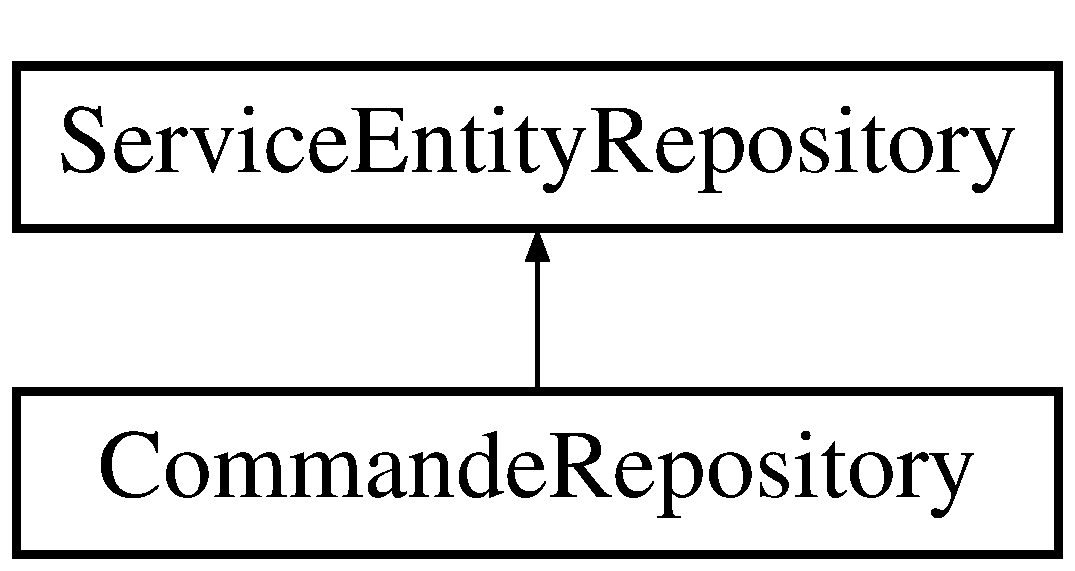
\includegraphics[height=2.000000cm]{class_app_1_1_repository_1_1_commande_repository}
\end{center}
\end{figure}
\subsection*{Public Member Functions}
\begin{DoxyCompactItemize}
\item 
\mbox{\hyperlink{class_app_1_1_repository_1_1_commande_repository_a38ea33dde11163765f358f5f10a3bc03}{\+\_\+\+\_\+construct}} (Manager\+Registry \$registry)
\end{DoxyCompactItemize}


\subsection{Detailed Description}
Commande$\vert$null find(\$id, \$lock\+Mode = null, \$lock\+Version = null)  Commande$\vert$null find\+One\+By(array \$criteria, array \$order\+By = null)  Commande\mbox{[}\mbox{]} find\+All()  Commande\mbox{[}\mbox{]} find\+By(array \$criteria, array \$order\+By = null, \$limit = null, \$offset = null) 

\subsection{Constructor \& Destructor Documentation}
\mbox{\Hypertarget{class_app_1_1_repository_1_1_commande_repository_a38ea33dde11163765f358f5f10a3bc03}\label{class_app_1_1_repository_1_1_commande_repository_a38ea33dde11163765f358f5f10a3bc03}} 
\index{App\+::\+Repository\+::\+Commande\+Repository@{App\+::\+Repository\+::\+Commande\+Repository}!\+\_\+\+\_\+construct@{\+\_\+\+\_\+construct}}
\index{\+\_\+\+\_\+construct@{\+\_\+\+\_\+construct}!App\+::\+Repository\+::\+Commande\+Repository@{App\+::\+Repository\+::\+Commande\+Repository}}
\subsubsection{\texorpdfstring{\+\_\+\+\_\+construct()}{\_\_construct()}}
{\footnotesize\ttfamily \+\_\+\+\_\+construct (\begin{DoxyParamCaption}\item[{Manager\+Registry}]{\$registry }\end{DoxyParamCaption})}



The documentation for this class was generated from the following file\+:\begin{DoxyCompactItemize}
\item 
src/\+Repository/\mbox{\hyperlink{_commande_repository_8php}{Commande\+Repository.\+php}}\end{DoxyCompactItemize}

\hypertarget{class_app_1_1_kernel}{}\section{Kernel Class Reference}
\label{class_app_1_1_kernel}\index{Kernel@{Kernel}}
Inheritance diagram for Kernel\+:\begin{figure}[H]
\begin{center}
\leavevmode
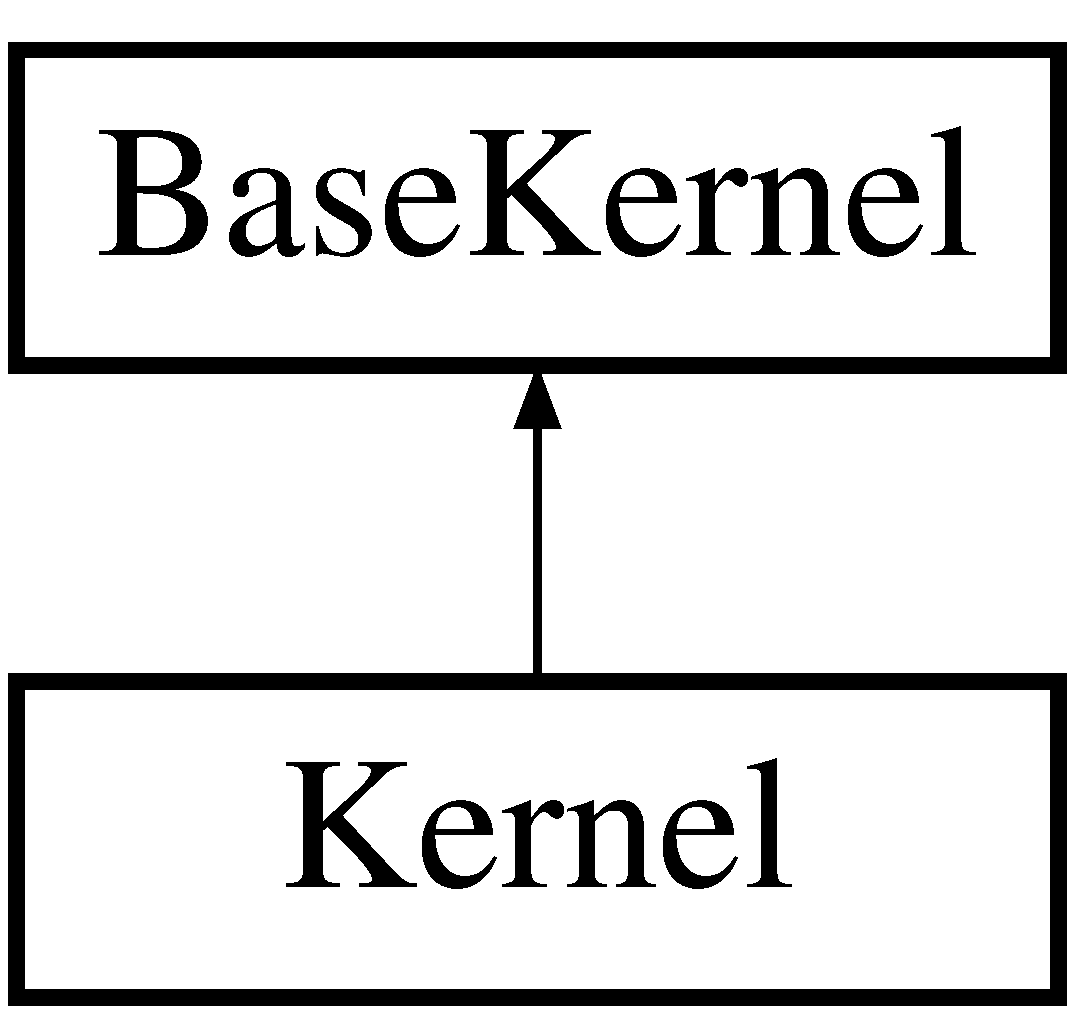
\includegraphics[height=2.000000cm]{class_app_1_1_kernel}
\end{center}
\end{figure}
\subsection*{Protected Member Functions}
\begin{DoxyCompactItemize}
\item 
\mbox{\hyperlink{class_app_1_1_kernel_a1776c0577417142eedd4b5693ad65546}{configure\+Container}} (Container\+Configurator \$container)
\item 
\mbox{\hyperlink{class_app_1_1_kernel_a8208f0c7a8a63568f8bae24547f3a666}{configure\+Routes}} (Routing\+Configurator \$routes)
\end{DoxyCompactItemize}


\subsection{Member Function Documentation}
\mbox{\Hypertarget{class_app_1_1_kernel_a1776c0577417142eedd4b5693ad65546}\label{class_app_1_1_kernel_a1776c0577417142eedd4b5693ad65546}} 
\index{App\+::\+Kernel@{App\+::\+Kernel}!configure\+Container@{configure\+Container}}
\index{configure\+Container@{configure\+Container}!App\+::\+Kernel@{App\+::\+Kernel}}
\subsubsection{\texorpdfstring{configure\+Container()}{configureContainer()}}
{\footnotesize\ttfamily configure\+Container (\begin{DoxyParamCaption}\item[{Container\+Configurator}]{\$container }\end{DoxyParamCaption})\hspace{0.3cm}{\ttfamily [protected]}}

\mbox{\Hypertarget{class_app_1_1_kernel_a8208f0c7a8a63568f8bae24547f3a666}\label{class_app_1_1_kernel_a8208f0c7a8a63568f8bae24547f3a666}} 
\index{App\+::\+Kernel@{App\+::\+Kernel}!configure\+Routes@{configure\+Routes}}
\index{configure\+Routes@{configure\+Routes}!App\+::\+Kernel@{App\+::\+Kernel}}
\subsubsection{\texorpdfstring{configure\+Routes()}{configureRoutes()}}
{\footnotesize\ttfamily configure\+Routes (\begin{DoxyParamCaption}\item[{Routing\+Configurator}]{\$routes }\end{DoxyParamCaption})\hspace{0.3cm}{\ttfamily [protected]}}



The documentation for this class was generated from the following file\+:\begin{DoxyCompactItemize}
\item 
src/\mbox{\hyperlink{_kernel_8php}{Kernel.\+php}}\end{DoxyCompactItemize}

\hypertarget{class_app_1_1_controller_1_1_mail_contact_controller}{}\section{Mail\+Contact\+Controller Class Reference}
\label{class_app_1_1_controller_1_1_mail_contact_controller}\index{Mail\+Contact\+Controller@{Mail\+Contact\+Controller}}
Inheritance diagram for Mail\+Contact\+Controller\+:\begin{figure}[H]
\begin{center}
\leavevmode
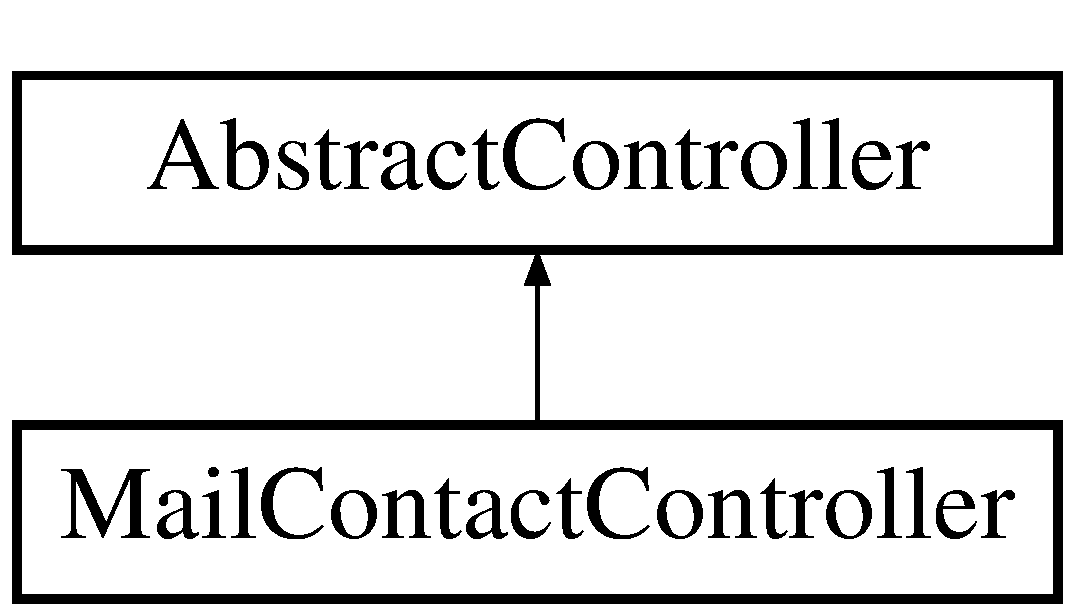
\includegraphics[height=2.000000cm]{class_app_1_1_controller_1_1_mail_contact_controller}
\end{center}
\end{figure}
\subsection*{Public Member Functions}
\begin{DoxyCompactItemize}
\item 
\mbox{\hyperlink{class_app_1_1_controller_1_1_mail_contact_controller_a1032c2b90260e3c85df9691126800ff2}{index}} (Request \$request, Mailer\+Interface \$mailer)
\end{DoxyCompactItemize}


\subsection{Detailed Description}
Manages the sending of mail \begin{DoxyAuthor}{Author}
Michael B\+E\+C\+Q\+U\+ER 
\end{DoxyAuthor}


\subsection{Member Function Documentation}
\mbox{\Hypertarget{class_app_1_1_controller_1_1_mail_contact_controller_a1032c2b90260e3c85df9691126800ff2}\label{class_app_1_1_controller_1_1_mail_contact_controller_a1032c2b90260e3c85df9691126800ff2}} 
\index{App\+::\+Controller\+::\+Mail\+Contact\+Controller@{App\+::\+Controller\+::\+Mail\+Contact\+Controller}!index@{index}}
\index{index@{index}!App\+::\+Controller\+::\+Mail\+Contact\+Controller@{App\+::\+Controller\+::\+Mail\+Contact\+Controller}}
\subsubsection{\texorpdfstring{index()}{index()}}
{\footnotesize\ttfamily index (\begin{DoxyParamCaption}\item[{Request}]{\$request,  }\item[{Mailer\+Interface}]{\$mailer }\end{DoxyParamCaption})}

(\char`\"{}/mail/contact\char`\"{}, name=\char`\"{}mail\+\_\+contact\char`\"{}) Sends a mail to the association


\begin{DoxyParams}[1]{Parameters}
mixed & {\em \$request} & \\
\hline
mixed & {\em \$mailer} & \\
\hline
\end{DoxyParams}
\begin{DoxyReturn}{Returns}
void 
\end{DoxyReturn}


The documentation for this class was generated from the following file\+:\begin{DoxyCompactItemize}
\item 
src/\+Controller/\mbox{\hyperlink{_mail_contact_controller_8php}{Mail\+Contact\+Controller.\+php}}\end{DoxyCompactItemize}

\hypertarget{class_app_1_1_entity_1_1_produits}{}\section{Produits Class Reference}
\label{class_app_1_1_entity_1_1_produits}\index{Produits@{Produits}}
\subsection*{Public Member Functions}
\begin{DoxyCompactItemize}
\item 
\mbox{\hyperlink{class_app_1_1_entity_1_1_produits_a095c5d389db211932136b53f25f39685}{\+\_\+\+\_\+construct}} ()
\item 
\mbox{\hyperlink{class_app_1_1_entity_1_1_produits_a12251d0c022e9e21c137a105ff683f13}{get\+Id}} ()
\item 
\mbox{\hyperlink{class_app_1_1_entity_1_1_produits_a184f2299ee4553fa0782ea87c9aed362}{get\+Nom}} ()
\item 
\mbox{\hyperlink{class_app_1_1_entity_1_1_produits_ad9079562ce21dfd57a8fb9cfe1e8f8ba}{set\+Nom}} (string \$nom)
\item 
\mbox{\hyperlink{class_app_1_1_entity_1_1_produits_a2af8add37797384585cae101fb8cbfe7}{get\+Image}} ()
\item 
\mbox{\hyperlink{class_app_1_1_entity_1_1_produits_acb73da7147aa4dbe762b5e438974bea9}{set\+Image}} (string \$image)
\item 
\mbox{\hyperlink{class_app_1_1_entity_1_1_produits_a36d5e4316fca03a6f45dc4554d86cb12}{get\+Prix}} ()
\item 
\mbox{\hyperlink{class_app_1_1_entity_1_1_produits_a85091a25a9a780dfb7dca7cbf27b3a92}{set\+Prix}} (float \$prix)
\item 
\mbox{\hyperlink{class_app_1_1_entity_1_1_produits_a8729ba486702e7e12a3fff08965e1e7f}{get\+Categories}} ()
\item 
\mbox{\hyperlink{class_app_1_1_entity_1_1_produits_aca93a29c7e12ee27f70c76e0a828c856}{add\+Category}} (\mbox{\hyperlink{class_app_1_1_entity_1_1_category}{Category}} \$category)
\item 
\mbox{\hyperlink{class_app_1_1_entity_1_1_produits_aa0568b366ced44f87b82aa00fe6ff1b7}{remove\+Category}} (\mbox{\hyperlink{class_app_1_1_entity_1_1_category}{Category}} \$category)
\item 
\mbox{\hyperlink{class_app_1_1_entity_1_1_produits_a0f0455d4aafe27d1b0720c3bcfff2847}{get\+Created\+At}} ()
\item 
\mbox{\hyperlink{class_app_1_1_entity_1_1_produits_a2308609ef549a753223bbee71e36291e}{set\+Created\+At}} (\textbackslash{}Date\+Time\+Interface \$created\+At)
\item 
\mbox{\hyperlink{class_app_1_1_entity_1_1_produits_af01723b72fddbef7e1529591b32ac96d}{get\+Carts}} ()
\item 
\mbox{\hyperlink{class_app_1_1_entity_1_1_produits_ae6fc61e1d99695b1cd2907cf4efef430}{add\+Cart}} (\mbox{\hyperlink{class_app_1_1_entity_1_1_cart}{Cart}} \$cart)
\item 
\mbox{\hyperlink{class_app_1_1_entity_1_1_produits_a9aff9e8abf19d0390713e9ead0968f85}{remove\+Cart}} (\mbox{\hyperlink{class_app_1_1_entity_1_1_cart}{Cart}} \$cart)
\end{DoxyCompactItemize}


\subsection{Detailed Description}
() (repository\+Class=Produits\+Repository\+::class) 

\subsection{Constructor \& Destructor Documentation}
\mbox{\Hypertarget{class_app_1_1_entity_1_1_produits_a095c5d389db211932136b53f25f39685}\label{class_app_1_1_entity_1_1_produits_a095c5d389db211932136b53f25f39685}} 
\index{App\+::\+Entity\+::\+Produits@{App\+::\+Entity\+::\+Produits}!\+\_\+\+\_\+construct@{\+\_\+\+\_\+construct}}
\index{\+\_\+\+\_\+construct@{\+\_\+\+\_\+construct}!App\+::\+Entity\+::\+Produits@{App\+::\+Entity\+::\+Produits}}
\subsubsection{\texorpdfstring{\+\_\+\+\_\+construct()}{\_\_construct()}}
{\footnotesize\ttfamily \+\_\+\+\_\+construct (\begin{DoxyParamCaption}{ }\end{DoxyParamCaption})}



\subsection{Member Function Documentation}
\mbox{\Hypertarget{class_app_1_1_entity_1_1_produits_ae6fc61e1d99695b1cd2907cf4efef430}\label{class_app_1_1_entity_1_1_produits_ae6fc61e1d99695b1cd2907cf4efef430}} 
\index{App\+::\+Entity\+::\+Produits@{App\+::\+Entity\+::\+Produits}!add\+Cart@{add\+Cart}}
\index{add\+Cart@{add\+Cart}!App\+::\+Entity\+::\+Produits@{App\+::\+Entity\+::\+Produits}}
\subsubsection{\texorpdfstring{add\+Cart()}{addCart()}}
{\footnotesize\ttfamily add\+Cart (\begin{DoxyParamCaption}\item[{\mbox{\hyperlink{class_app_1_1_entity_1_1_cart}{Cart}}}]{\$cart }\end{DoxyParamCaption})}

\mbox{\Hypertarget{class_app_1_1_entity_1_1_produits_aca93a29c7e12ee27f70c76e0a828c856}\label{class_app_1_1_entity_1_1_produits_aca93a29c7e12ee27f70c76e0a828c856}} 
\index{App\+::\+Entity\+::\+Produits@{App\+::\+Entity\+::\+Produits}!add\+Category@{add\+Category}}
\index{add\+Category@{add\+Category}!App\+::\+Entity\+::\+Produits@{App\+::\+Entity\+::\+Produits}}
\subsubsection{\texorpdfstring{add\+Category()}{addCategory()}}
{\footnotesize\ttfamily add\+Category (\begin{DoxyParamCaption}\item[{\mbox{\hyperlink{class_app_1_1_entity_1_1_category}{Category}}}]{\$category }\end{DoxyParamCaption})}

\mbox{\Hypertarget{class_app_1_1_entity_1_1_produits_af01723b72fddbef7e1529591b32ac96d}\label{class_app_1_1_entity_1_1_produits_af01723b72fddbef7e1529591b32ac96d}} 
\index{App\+::\+Entity\+::\+Produits@{App\+::\+Entity\+::\+Produits}!get\+Carts@{get\+Carts}}
\index{get\+Carts@{get\+Carts}!App\+::\+Entity\+::\+Produits@{App\+::\+Entity\+::\+Produits}}
\subsubsection{\texorpdfstring{get\+Carts()}{getCarts()}}
{\footnotesize\ttfamily get\+Carts (\begin{DoxyParamCaption}{ }\end{DoxyParamCaption})}

\begin{DoxyReturn}{Returns}
Collection$\vert$\+Cart\mbox{[}\mbox{]} 
\end{DoxyReturn}
\mbox{\Hypertarget{class_app_1_1_entity_1_1_produits_a8729ba486702e7e12a3fff08965e1e7f}\label{class_app_1_1_entity_1_1_produits_a8729ba486702e7e12a3fff08965e1e7f}} 
\index{App\+::\+Entity\+::\+Produits@{App\+::\+Entity\+::\+Produits}!get\+Categories@{get\+Categories}}
\index{get\+Categories@{get\+Categories}!App\+::\+Entity\+::\+Produits@{App\+::\+Entity\+::\+Produits}}
\subsubsection{\texorpdfstring{get\+Categories()}{getCategories()}}
{\footnotesize\ttfamily get\+Categories (\begin{DoxyParamCaption}{ }\end{DoxyParamCaption})}

\begin{DoxyReturn}{Returns}
Collection$\vert$\+Category\mbox{[}\mbox{]} 
\end{DoxyReturn}
\mbox{\Hypertarget{class_app_1_1_entity_1_1_produits_a0f0455d4aafe27d1b0720c3bcfff2847}\label{class_app_1_1_entity_1_1_produits_a0f0455d4aafe27d1b0720c3bcfff2847}} 
\index{App\+::\+Entity\+::\+Produits@{App\+::\+Entity\+::\+Produits}!get\+Created\+At@{get\+Created\+At}}
\index{get\+Created\+At@{get\+Created\+At}!App\+::\+Entity\+::\+Produits@{App\+::\+Entity\+::\+Produits}}
\subsubsection{\texorpdfstring{get\+Created\+At()}{getCreatedAt()}}
{\footnotesize\ttfamily get\+Created\+At (\begin{DoxyParamCaption}{ }\end{DoxyParamCaption})}

\mbox{\Hypertarget{class_app_1_1_entity_1_1_produits_a12251d0c022e9e21c137a105ff683f13}\label{class_app_1_1_entity_1_1_produits_a12251d0c022e9e21c137a105ff683f13}} 
\index{App\+::\+Entity\+::\+Produits@{App\+::\+Entity\+::\+Produits}!get\+Id@{get\+Id}}
\index{get\+Id@{get\+Id}!App\+::\+Entity\+::\+Produits@{App\+::\+Entity\+::\+Produits}}
\subsubsection{\texorpdfstring{get\+Id()}{getId()}}
{\footnotesize\ttfamily get\+Id (\begin{DoxyParamCaption}{ }\end{DoxyParamCaption})}

\mbox{\Hypertarget{class_app_1_1_entity_1_1_produits_a2af8add37797384585cae101fb8cbfe7}\label{class_app_1_1_entity_1_1_produits_a2af8add37797384585cae101fb8cbfe7}} 
\index{App\+::\+Entity\+::\+Produits@{App\+::\+Entity\+::\+Produits}!get\+Image@{get\+Image}}
\index{get\+Image@{get\+Image}!App\+::\+Entity\+::\+Produits@{App\+::\+Entity\+::\+Produits}}
\subsubsection{\texorpdfstring{get\+Image()}{getImage()}}
{\footnotesize\ttfamily get\+Image (\begin{DoxyParamCaption}{ }\end{DoxyParamCaption})}

\mbox{\Hypertarget{class_app_1_1_entity_1_1_produits_a184f2299ee4553fa0782ea87c9aed362}\label{class_app_1_1_entity_1_1_produits_a184f2299ee4553fa0782ea87c9aed362}} 
\index{App\+::\+Entity\+::\+Produits@{App\+::\+Entity\+::\+Produits}!get\+Nom@{get\+Nom}}
\index{get\+Nom@{get\+Nom}!App\+::\+Entity\+::\+Produits@{App\+::\+Entity\+::\+Produits}}
\subsubsection{\texorpdfstring{get\+Nom()}{getNom()}}
{\footnotesize\ttfamily get\+Nom (\begin{DoxyParamCaption}{ }\end{DoxyParamCaption})}

\mbox{\Hypertarget{class_app_1_1_entity_1_1_produits_a36d5e4316fca03a6f45dc4554d86cb12}\label{class_app_1_1_entity_1_1_produits_a36d5e4316fca03a6f45dc4554d86cb12}} 
\index{App\+::\+Entity\+::\+Produits@{App\+::\+Entity\+::\+Produits}!get\+Prix@{get\+Prix}}
\index{get\+Prix@{get\+Prix}!App\+::\+Entity\+::\+Produits@{App\+::\+Entity\+::\+Produits}}
\subsubsection{\texorpdfstring{get\+Prix()}{getPrix()}}
{\footnotesize\ttfamily get\+Prix (\begin{DoxyParamCaption}{ }\end{DoxyParamCaption})}

\mbox{\Hypertarget{class_app_1_1_entity_1_1_produits_a9aff9e8abf19d0390713e9ead0968f85}\label{class_app_1_1_entity_1_1_produits_a9aff9e8abf19d0390713e9ead0968f85}} 
\index{App\+::\+Entity\+::\+Produits@{App\+::\+Entity\+::\+Produits}!remove\+Cart@{remove\+Cart}}
\index{remove\+Cart@{remove\+Cart}!App\+::\+Entity\+::\+Produits@{App\+::\+Entity\+::\+Produits}}
\subsubsection{\texorpdfstring{remove\+Cart()}{removeCart()}}
{\footnotesize\ttfamily remove\+Cart (\begin{DoxyParamCaption}\item[{\mbox{\hyperlink{class_app_1_1_entity_1_1_cart}{Cart}}}]{\$cart }\end{DoxyParamCaption})}

\mbox{\Hypertarget{class_app_1_1_entity_1_1_produits_aa0568b366ced44f87b82aa00fe6ff1b7}\label{class_app_1_1_entity_1_1_produits_aa0568b366ced44f87b82aa00fe6ff1b7}} 
\index{App\+::\+Entity\+::\+Produits@{App\+::\+Entity\+::\+Produits}!remove\+Category@{remove\+Category}}
\index{remove\+Category@{remove\+Category}!App\+::\+Entity\+::\+Produits@{App\+::\+Entity\+::\+Produits}}
\subsubsection{\texorpdfstring{remove\+Category()}{removeCategory()}}
{\footnotesize\ttfamily remove\+Category (\begin{DoxyParamCaption}\item[{\mbox{\hyperlink{class_app_1_1_entity_1_1_category}{Category}}}]{\$category }\end{DoxyParamCaption})}

\mbox{\Hypertarget{class_app_1_1_entity_1_1_produits_a2308609ef549a753223bbee71e36291e}\label{class_app_1_1_entity_1_1_produits_a2308609ef549a753223bbee71e36291e}} 
\index{App\+::\+Entity\+::\+Produits@{App\+::\+Entity\+::\+Produits}!set\+Created\+At@{set\+Created\+At}}
\index{set\+Created\+At@{set\+Created\+At}!App\+::\+Entity\+::\+Produits@{App\+::\+Entity\+::\+Produits}}
\subsubsection{\texorpdfstring{set\+Created\+At()}{setCreatedAt()}}
{\footnotesize\ttfamily set\+Created\+At (\begin{DoxyParamCaption}\item[{\textbackslash{}Date\+Time\+Interface}]{\$created\+At }\end{DoxyParamCaption})}

\mbox{\Hypertarget{class_app_1_1_entity_1_1_produits_acb73da7147aa4dbe762b5e438974bea9}\label{class_app_1_1_entity_1_1_produits_acb73da7147aa4dbe762b5e438974bea9}} 
\index{App\+::\+Entity\+::\+Produits@{App\+::\+Entity\+::\+Produits}!set\+Image@{set\+Image}}
\index{set\+Image@{set\+Image}!App\+::\+Entity\+::\+Produits@{App\+::\+Entity\+::\+Produits}}
\subsubsection{\texorpdfstring{set\+Image()}{setImage()}}
{\footnotesize\ttfamily set\+Image (\begin{DoxyParamCaption}\item[{string}]{\$image }\end{DoxyParamCaption})}

\mbox{\Hypertarget{class_app_1_1_entity_1_1_produits_ad9079562ce21dfd57a8fb9cfe1e8f8ba}\label{class_app_1_1_entity_1_1_produits_ad9079562ce21dfd57a8fb9cfe1e8f8ba}} 
\index{App\+::\+Entity\+::\+Produits@{App\+::\+Entity\+::\+Produits}!set\+Nom@{set\+Nom}}
\index{set\+Nom@{set\+Nom}!App\+::\+Entity\+::\+Produits@{App\+::\+Entity\+::\+Produits}}
\subsubsection{\texorpdfstring{set\+Nom()}{setNom()}}
{\footnotesize\ttfamily set\+Nom (\begin{DoxyParamCaption}\item[{string}]{\$nom }\end{DoxyParamCaption})}

\mbox{\Hypertarget{class_app_1_1_entity_1_1_produits_a85091a25a9a780dfb7dca7cbf27b3a92}\label{class_app_1_1_entity_1_1_produits_a85091a25a9a780dfb7dca7cbf27b3a92}} 
\index{App\+::\+Entity\+::\+Produits@{App\+::\+Entity\+::\+Produits}!set\+Prix@{set\+Prix}}
\index{set\+Prix@{set\+Prix}!App\+::\+Entity\+::\+Produits@{App\+::\+Entity\+::\+Produits}}
\subsubsection{\texorpdfstring{set\+Prix()}{setPrix()}}
{\footnotesize\ttfamily set\+Prix (\begin{DoxyParamCaption}\item[{float}]{\$prix }\end{DoxyParamCaption})}



The documentation for this class was generated from the following file\+:\begin{DoxyCompactItemize}
\item 
src/\+Entity/\mbox{\hyperlink{_produits_8php}{Produits.\+php}}\end{DoxyCompactItemize}

\hypertarget{class_app_1_1_repository_1_1_produits_repository}{}\section{Produits\+Repository Class Reference}
\label{class_app_1_1_repository_1_1_produits_repository}\index{Produits\+Repository@{Produits\+Repository}}
Inheritance diagram for Produits\+Repository\+:\begin{figure}[H]
\begin{center}
\leavevmode
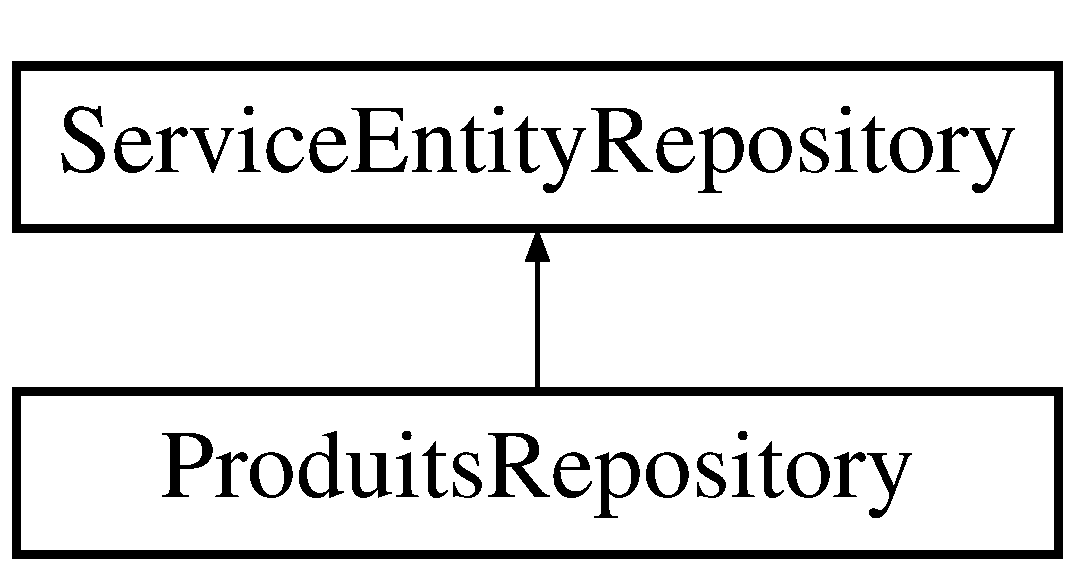
\includegraphics[height=2.000000cm]{class_app_1_1_repository_1_1_produits_repository}
\end{center}
\end{figure}
\subsection*{Public Member Functions}
\begin{DoxyCompactItemize}
\item 
\mbox{\hyperlink{class_app_1_1_repository_1_1_produits_repository_a38ea33dde11163765f358f5f10a3bc03}{\+\_\+\+\_\+construct}} (Manager\+Registry \$registry)
\end{DoxyCompactItemize}


\subsection{Detailed Description}
Produits$\vert$null find(\$id, \$lock\+Mode = null, \$lock\+Version = null)  Produits$\vert$null find\+One\+By(array \$criteria, array \$order\+By = null)  Produits\mbox{[}\mbox{]} find\+All()  Produits\mbox{[}\mbox{]} find\+By(array \$criteria, array \$order\+By = null, \$limit = null, \$offset = null) 

\subsection{Constructor \& Destructor Documentation}
\mbox{\Hypertarget{class_app_1_1_repository_1_1_produits_repository_a38ea33dde11163765f358f5f10a3bc03}\label{class_app_1_1_repository_1_1_produits_repository_a38ea33dde11163765f358f5f10a3bc03}} 
\index{App\+::\+Repository\+::\+Produits\+Repository@{App\+::\+Repository\+::\+Produits\+Repository}!\+\_\+\+\_\+construct@{\+\_\+\+\_\+construct}}
\index{\+\_\+\+\_\+construct@{\+\_\+\+\_\+construct}!App\+::\+Repository\+::\+Produits\+Repository@{App\+::\+Repository\+::\+Produits\+Repository}}
\subsubsection{\texorpdfstring{\+\_\+\+\_\+construct()}{\_\_construct()}}
{\footnotesize\ttfamily \+\_\+\+\_\+construct (\begin{DoxyParamCaption}\item[{Manager\+Registry}]{\$registry }\end{DoxyParamCaption})}



The documentation for this class was generated from the following file\+:\begin{DoxyCompactItemize}
\item 
src/\+Repository/\mbox{\hyperlink{_produits_repository_8php}{Produits\+Repository.\+php}}\end{DoxyCompactItemize}

\hypertarget{class_app_1_1_entity_1_1_role}{}\section{Role Class Reference}
\label{class_app_1_1_entity_1_1_role}\index{Role@{Role}}
\subsection*{Public Member Functions}
\begin{DoxyCompactItemize}
\item 
\mbox{\hyperlink{class_app_1_1_entity_1_1_role_a095c5d389db211932136b53f25f39685}{\+\_\+\+\_\+construct}} ()
\item 
\mbox{\hyperlink{class_app_1_1_entity_1_1_role_a12251d0c022e9e21c137a105ff683f13}{get\+Id}} ()
\item 
\mbox{\hyperlink{class_app_1_1_entity_1_1_role_a0fc10b64683021b70c7eb95fb514c119}{get\+Users}} ()
\item 
\mbox{\hyperlink{class_app_1_1_entity_1_1_role_a79440b2b582b2ea5990f400faf2c8293}{add\+Users}} (\mbox{\hyperlink{class_app_1_1_entity_1_1_users}{Users}} \$user)
\item 
\mbox{\hyperlink{class_app_1_1_entity_1_1_role_a1432bc398227897369e3cc1874a2ec17}{remove\+Users}} (\mbox{\hyperlink{class_app_1_1_entity_1_1_users}{Users}} \$user)
\item 
\mbox{\hyperlink{class_app_1_1_entity_1_1_role_a3d0963e68bb313b163a73f2803c64600}{get\+Name}} ()
\item 
\mbox{\hyperlink{class_app_1_1_entity_1_1_role_a392752b62c4f6aacea5c269690921ef3}{set\+Name}} (string \$name)
\end{DoxyCompactItemize}


\subsection{Detailed Description}
() (repository\+Class=Role\+Repository\+::class) 

\subsection{Constructor \& Destructor Documentation}
\mbox{\Hypertarget{class_app_1_1_entity_1_1_role_a095c5d389db211932136b53f25f39685}\label{class_app_1_1_entity_1_1_role_a095c5d389db211932136b53f25f39685}} 
\index{App\+::\+Entity\+::\+Role@{App\+::\+Entity\+::\+Role}!\+\_\+\+\_\+construct@{\+\_\+\+\_\+construct}}
\index{\+\_\+\+\_\+construct@{\+\_\+\+\_\+construct}!App\+::\+Entity\+::\+Role@{App\+::\+Entity\+::\+Role}}
\subsubsection{\texorpdfstring{\+\_\+\+\_\+construct()}{\_\_construct()}}
{\footnotesize\ttfamily \+\_\+\+\_\+construct (\begin{DoxyParamCaption}{ }\end{DoxyParamCaption})}



\subsection{Member Function Documentation}
\mbox{\Hypertarget{class_app_1_1_entity_1_1_role_a79440b2b582b2ea5990f400faf2c8293}\label{class_app_1_1_entity_1_1_role_a79440b2b582b2ea5990f400faf2c8293}} 
\index{App\+::\+Entity\+::\+Role@{App\+::\+Entity\+::\+Role}!add\+Users@{add\+Users}}
\index{add\+Users@{add\+Users}!App\+::\+Entity\+::\+Role@{App\+::\+Entity\+::\+Role}}
\subsubsection{\texorpdfstring{add\+Users()}{addUsers()}}
{\footnotesize\ttfamily add\+Users (\begin{DoxyParamCaption}\item[{\mbox{\hyperlink{class_app_1_1_entity_1_1_users}{Users}}}]{\$user }\end{DoxyParamCaption})}

\mbox{\Hypertarget{class_app_1_1_entity_1_1_role_a12251d0c022e9e21c137a105ff683f13}\label{class_app_1_1_entity_1_1_role_a12251d0c022e9e21c137a105ff683f13}} 
\index{App\+::\+Entity\+::\+Role@{App\+::\+Entity\+::\+Role}!get\+Id@{get\+Id}}
\index{get\+Id@{get\+Id}!App\+::\+Entity\+::\+Role@{App\+::\+Entity\+::\+Role}}
\subsubsection{\texorpdfstring{get\+Id()}{getId()}}
{\footnotesize\ttfamily get\+Id (\begin{DoxyParamCaption}{ }\end{DoxyParamCaption})}

\mbox{\Hypertarget{class_app_1_1_entity_1_1_role_a3d0963e68bb313b163a73f2803c64600}\label{class_app_1_1_entity_1_1_role_a3d0963e68bb313b163a73f2803c64600}} 
\index{App\+::\+Entity\+::\+Role@{App\+::\+Entity\+::\+Role}!get\+Name@{get\+Name}}
\index{get\+Name@{get\+Name}!App\+::\+Entity\+::\+Role@{App\+::\+Entity\+::\+Role}}
\subsubsection{\texorpdfstring{get\+Name()}{getName()}}
{\footnotesize\ttfamily get\+Name (\begin{DoxyParamCaption}{ }\end{DoxyParamCaption})}

\mbox{\Hypertarget{class_app_1_1_entity_1_1_role_a0fc10b64683021b70c7eb95fb514c119}\label{class_app_1_1_entity_1_1_role_a0fc10b64683021b70c7eb95fb514c119}} 
\index{App\+::\+Entity\+::\+Role@{App\+::\+Entity\+::\+Role}!get\+Users@{get\+Users}}
\index{get\+Users@{get\+Users}!App\+::\+Entity\+::\+Role@{App\+::\+Entity\+::\+Role}}
\subsubsection{\texorpdfstring{get\+Users()}{getUsers()}}
{\footnotesize\ttfamily get\+Users (\begin{DoxyParamCaption}{ }\end{DoxyParamCaption})}

\begin{DoxyReturn}{Returns}
Collection$\vert$\+Users\mbox{[}\mbox{]} 
\end{DoxyReturn}
\mbox{\Hypertarget{class_app_1_1_entity_1_1_role_a1432bc398227897369e3cc1874a2ec17}\label{class_app_1_1_entity_1_1_role_a1432bc398227897369e3cc1874a2ec17}} 
\index{App\+::\+Entity\+::\+Role@{App\+::\+Entity\+::\+Role}!remove\+Users@{remove\+Users}}
\index{remove\+Users@{remove\+Users}!App\+::\+Entity\+::\+Role@{App\+::\+Entity\+::\+Role}}
\subsubsection{\texorpdfstring{remove\+Users()}{removeUsers()}}
{\footnotesize\ttfamily remove\+Users (\begin{DoxyParamCaption}\item[{\mbox{\hyperlink{class_app_1_1_entity_1_1_users}{Users}}}]{\$user }\end{DoxyParamCaption})}

\mbox{\Hypertarget{class_app_1_1_entity_1_1_role_a392752b62c4f6aacea5c269690921ef3}\label{class_app_1_1_entity_1_1_role_a392752b62c4f6aacea5c269690921ef3}} 
\index{App\+::\+Entity\+::\+Role@{App\+::\+Entity\+::\+Role}!set\+Name@{set\+Name}}
\index{set\+Name@{set\+Name}!App\+::\+Entity\+::\+Role@{App\+::\+Entity\+::\+Role}}
\subsubsection{\texorpdfstring{set\+Name()}{setName()}}
{\footnotesize\ttfamily set\+Name (\begin{DoxyParamCaption}\item[{string}]{\$name }\end{DoxyParamCaption})}



The documentation for this class was generated from the following file\+:\begin{DoxyCompactItemize}
\item 
src/\+Entity/\mbox{\hyperlink{_role_8php}{Role.\+php}}\end{DoxyCompactItemize}

\hypertarget{class_app_1_1_repository_1_1_role_repository}{}\section{Role\+Repository Class Reference}
\label{class_app_1_1_repository_1_1_role_repository}\index{Role\+Repository@{Role\+Repository}}
Inheritance diagram for Role\+Repository\+:\begin{figure}[H]
\begin{center}
\leavevmode
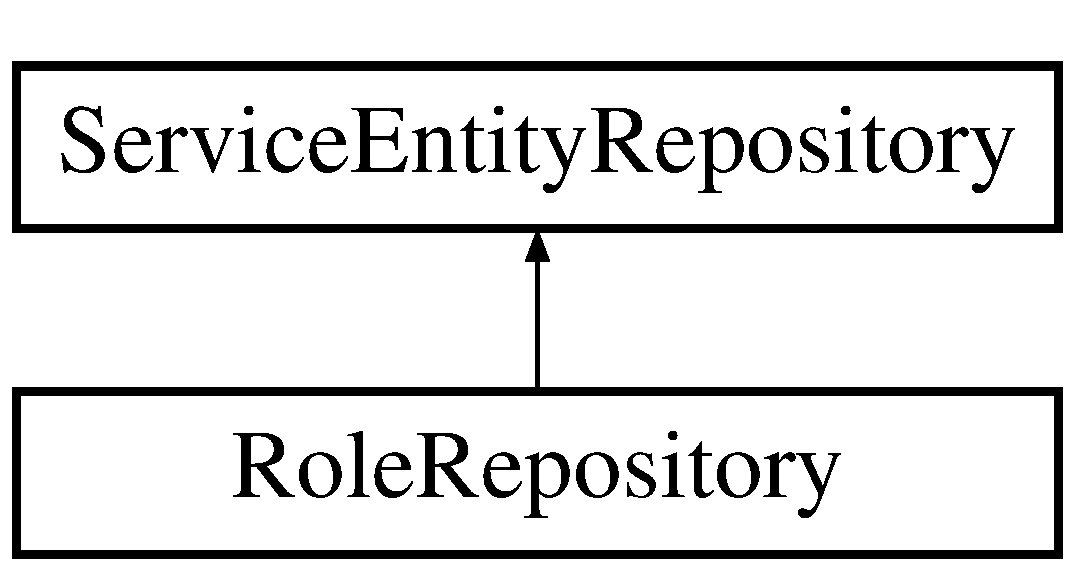
\includegraphics[height=2.000000cm]{class_app_1_1_repository_1_1_role_repository}
\end{center}
\end{figure}
\subsection*{Public Member Functions}
\begin{DoxyCompactItemize}
\item 
\mbox{\hyperlink{class_app_1_1_repository_1_1_role_repository_a38ea33dde11163765f358f5f10a3bc03}{\+\_\+\+\_\+construct}} (Manager\+Registry \$registry)
\end{DoxyCompactItemize}


\subsection{Detailed Description}
Role$\vert$null find(\$id, \$lock\+Mode = null, \$lock\+Version = null)  Role$\vert$null find\+One\+By(array \$criteria, array \$order\+By = null)  Role\mbox{[}\mbox{]} find\+All()  Role\mbox{[}\mbox{]} find\+By(array \$criteria, array \$order\+By = null, \$limit = null, \$offset = null) 

\subsection{Constructor \& Destructor Documentation}
\mbox{\Hypertarget{class_app_1_1_repository_1_1_role_repository_a38ea33dde11163765f358f5f10a3bc03}\label{class_app_1_1_repository_1_1_role_repository_a38ea33dde11163765f358f5f10a3bc03}} 
\index{App\+::\+Repository\+::\+Role\+Repository@{App\+::\+Repository\+::\+Role\+Repository}!\+\_\+\+\_\+construct@{\+\_\+\+\_\+construct}}
\index{\+\_\+\+\_\+construct@{\+\_\+\+\_\+construct}!App\+::\+Repository\+::\+Role\+Repository@{App\+::\+Repository\+::\+Role\+Repository}}
\subsubsection{\texorpdfstring{\+\_\+\+\_\+construct()}{\_\_construct()}}
{\footnotesize\ttfamily \+\_\+\+\_\+construct (\begin{DoxyParamCaption}\item[{Manager\+Registry}]{\$registry }\end{DoxyParamCaption})}



The documentation for this class was generated from the following file\+:\begin{DoxyCompactItemize}
\item 
src/\+Repository/\mbox{\hyperlink{_role_repository_8php}{Role\+Repository.\+php}}\end{DoxyCompactItemize}

\hypertarget{class_app_1_1_controller_1_1_user_controller}{}\section{User\+Controller Class Reference}
\label{class_app_1_1_controller_1_1_user_controller}\index{User\+Controller@{User\+Controller}}
Inheritance diagram for User\+Controller\+:\begin{figure}[H]
\begin{center}
\leavevmode
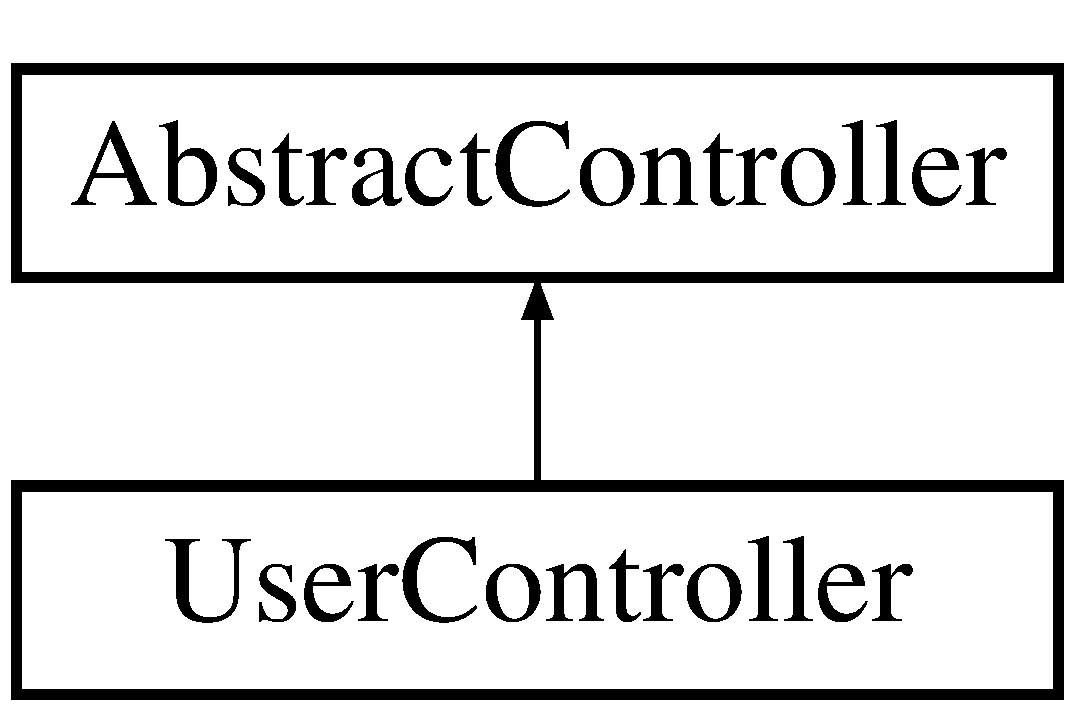
\includegraphics[height=2.000000cm]{class_app_1_1_controller_1_1_user_controller}
\end{center}
\end{figure}
\subsection*{Public Member Functions}
\begin{DoxyCompactItemize}
\item 
\mbox{\hyperlink{class_app_1_1_controller_1_1_user_controller_a18d2b8ef36c20c54ff76c6ce68534409}{index}} (Request \$request, Entity\+Manager\+Interface \$manager, User\+Password\+Encoder\+Interface \$encoder, Validator\+Interface \$validator, \mbox{\hyperlink{class_app_1_1_repository_1_1_role_repository}{Role\+Repository}} \$role\+Repository)
\item 
\mbox{\hyperlink{class_app_1_1_controller_1_1_user_controller_affba077e60f5a9a813c6880603500ec5}{login\+Check}} ()
\end{DoxyCompactItemize}


\subsection{Detailed Description}
Manages user registration and login \begin{DoxyAuthor}{Author}
Michael B\+E\+C\+Q\+U\+ER 
\end{DoxyAuthor}


\subsection{Member Function Documentation}
\mbox{\Hypertarget{class_app_1_1_controller_1_1_user_controller_a18d2b8ef36c20c54ff76c6ce68534409}\label{class_app_1_1_controller_1_1_user_controller_a18d2b8ef36c20c54ff76c6ce68534409}} 
\index{App\+::\+Controller\+::\+User\+Controller@{App\+::\+Controller\+::\+User\+Controller}!index@{index}}
\index{index@{index}!App\+::\+Controller\+::\+User\+Controller@{App\+::\+Controller\+::\+User\+Controller}}
\subsubsection{\texorpdfstring{index()}{index()}}
{\footnotesize\ttfamily index (\begin{DoxyParamCaption}\item[{Request}]{\$request,  }\item[{Entity\+Manager\+Interface}]{\$manager,  }\item[{User\+Password\+Encoder\+Interface}]{\$encoder,  }\item[{Validator\+Interface}]{\$validator,  }\item[{\mbox{\hyperlink{class_app_1_1_repository_1_1_role_repository}{Role\+Repository}}}]{\$role\+Repository }\end{DoxyParamCaption})}

(\char`\"{}/register\char`\"{}, name=\char`\"{}register\char`\"{}, methods=\{\char`\"{}\+P\+O\+S\+T\char`\"{}\}) Register a user in the database


\begin{DoxyParams}[1]{Parameters}
mixed & {\em \$request} & \\
\hline
mixed & {\em \$manager} & \\
\hline
mixed & {\em \$encoder} & \\
\hline
mixed & {\em \$validator} & \\
\hline
mixed & {\em \$role\+Repository} & \\
\hline
\end{DoxyParams}
\begin{DoxyReturn}{Returns}
response 
\end{DoxyReturn}
Uses a \+\_\+\+\_\+to\+String method on the \$errors variable which is a Constraint\+Violation\+List object. This gives us a nice string for debugging.\mbox{\Hypertarget{class_app_1_1_controller_1_1_user_controller_affba077e60f5a9a813c6880603500ec5}\label{class_app_1_1_controller_1_1_user_controller_affba077e60f5a9a813c6880603500ec5}} 
\index{App\+::\+Controller\+::\+User\+Controller@{App\+::\+Controller\+::\+User\+Controller}!login\+Check@{login\+Check}}
\index{login\+Check@{login\+Check}!App\+::\+Controller\+::\+User\+Controller@{App\+::\+Controller\+::\+User\+Controller}}
\subsubsection{\texorpdfstring{login\+Check()}{loginCheck()}}
{\footnotesize\ttfamily login\+Check (\begin{DoxyParamCaption}{ }\end{DoxyParamCaption})}

(\char`\"{}/api/login\+\_\+check\char`\"{}, name=\char`\"{}api\+\_\+login\+\_\+check\char`\"{}, methods=\{\char`\"{}\+P\+O\+S\+T\char`\"{}\}) Enable to check if user is connected to database

\begin{DoxyReturn}{Returns}
Json\+Response 
\end{DoxyReturn}


The documentation for this class was generated from the following file\+:\begin{DoxyCompactItemize}
\item 
src/\+Controller/\mbox{\hyperlink{_user_controller_8php}{User\+Controller.\+php}}\end{DoxyCompactItemize}

\hypertarget{class_app_1_1_entity_1_1_users}{}\section{Users Class Reference}
\label{class_app_1_1_entity_1_1_users}\index{Users@{Users}}
Inheritance diagram for Users\+:\begin{figure}[H]
\begin{center}
\leavevmode
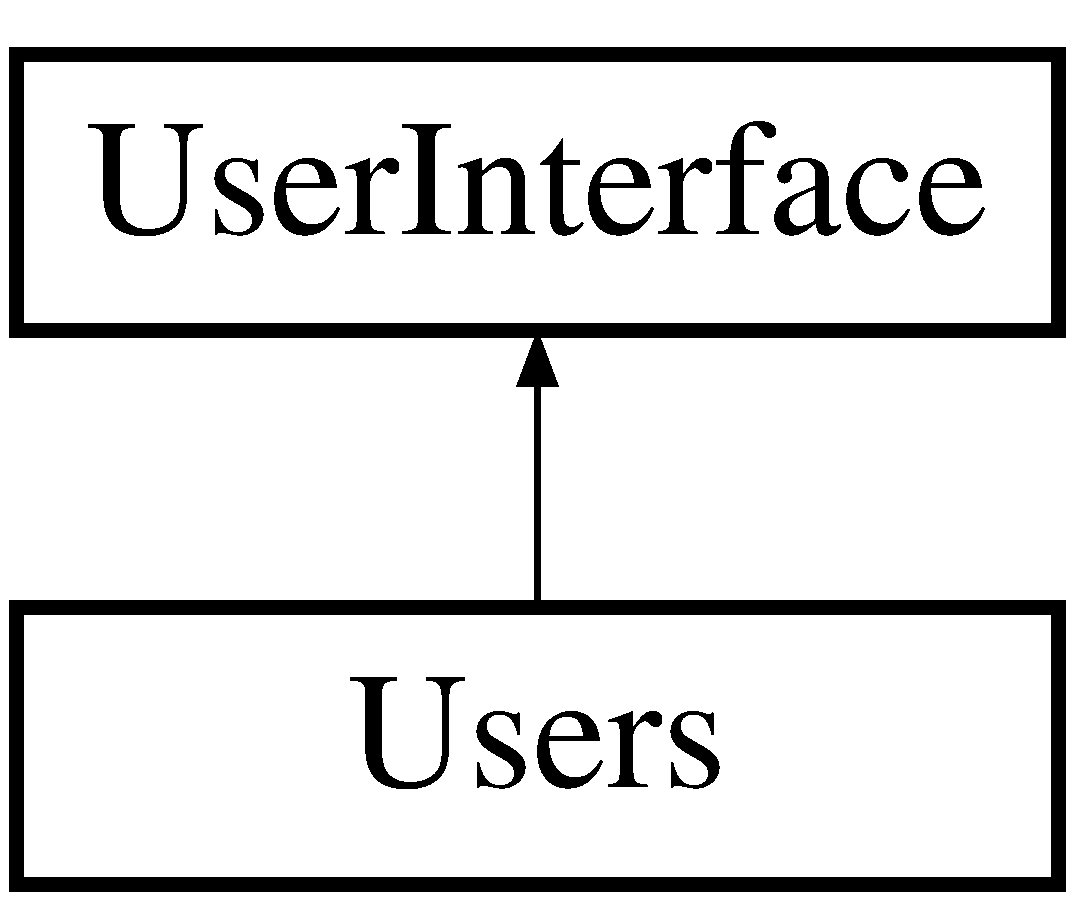
\includegraphics[height=2.000000cm]{class_app_1_1_entity_1_1_users}
\end{center}
\end{figure}
\subsection*{Public Member Functions}
\begin{DoxyCompactItemize}
\item 
\mbox{\hyperlink{class_app_1_1_entity_1_1_users_a095c5d389db211932136b53f25f39685}{\+\_\+\+\_\+construct}} ()
\item 
\mbox{\hyperlink{class_app_1_1_entity_1_1_users_a12251d0c022e9e21c137a105ff683f13}{get\+Id}} ()
\item 
\mbox{\hyperlink{class_app_1_1_entity_1_1_users_a02a01849f28e2535e888ae4ec87b20f2}{get\+Email}} ()
\item 
\mbox{\hyperlink{class_app_1_1_entity_1_1_users_a2d22391fa86fa0eaf3b9d2a3c29880bc}{set\+Email}} (string \$email)
\item 
\mbox{\hyperlink{class_app_1_1_entity_1_1_users_a81b37a3c9d639574e394f80c1138c75e}{get\+Username}} ()
\item 
\mbox{\hyperlink{class_app_1_1_entity_1_1_users_a499316b2a4d41cd073ad9ac7ece47b3a}{add\+Role}} (\mbox{\hyperlink{class_app_1_1_entity_1_1_role}{Role}} \$role)
\item 
\mbox{\hyperlink{class_app_1_1_entity_1_1_users_af336604c8c29aedc9c573c8499bce742}{remove\+Role}} (\mbox{\hyperlink{class_app_1_1_entity_1_1_role}{Role}} \$role)
\item 
\mbox{\hyperlink{class_app_1_1_entity_1_1_users_aa676cae5ee8d7fb6862a8724adc2660d}{get\+Roles}} ()
\item 
\mbox{\hyperlink{class_app_1_1_entity_1_1_users_a04e0957baeb7acde9c0c86556da2d43f}{get\+Password}} ()
\item 
\mbox{\hyperlink{class_app_1_1_entity_1_1_users_a1dfe56d2c965d451a135f3f3910a8b8d}{get\+Salt}} ()
\item 
\mbox{\hyperlink{class_app_1_1_entity_1_1_users_ac565b8c00fe93ce673f8237849f072a6}{erase\+Credentials}} ()
\item 
\mbox{\hyperlink{class_app_1_1_entity_1_1_users_a184f2299ee4553fa0782ea87c9aed362}{get\+Nom}} ()
\item 
\mbox{\hyperlink{class_app_1_1_entity_1_1_users_ad9079562ce21dfd57a8fb9cfe1e8f8ba}{set\+Nom}} (string \$nom)
\item 
\mbox{\hyperlink{class_app_1_1_entity_1_1_users_a0fb99b0610e269ca6409dd3a767ad8bf}{get\+Commandes}} ()
\item 
\mbox{\hyperlink{class_app_1_1_entity_1_1_users_a2872312b16486646f997c6c8fd579cca}{add\+Commande}} (\mbox{\hyperlink{class_app_1_1_entity_1_1_commande}{Commande}} \$commande)
\item 
\mbox{\hyperlink{class_app_1_1_entity_1_1_users_a98184ff8c042500a02552ee0cc6e305b}{remove\+Commande}} (\mbox{\hyperlink{class_app_1_1_entity_1_1_commande}{Commande}} \$commande)
\item 
\mbox{\hyperlink{class_app_1_1_entity_1_1_users_a81e0f429784973551fb5417d5b92b0db}{set\+Password}} (string \$password)
\item 
\mbox{\hyperlink{class_app_1_1_entity_1_1_users_af01723b72fddbef7e1529591b32ac96d}{get\+Carts}} ()
\item 
\mbox{\hyperlink{class_app_1_1_entity_1_1_users_ae6fc61e1d99695b1cd2907cf4efef430}{add\+Cart}} (\mbox{\hyperlink{class_app_1_1_entity_1_1_cart}{Cart}} \$cart)
\item 
\mbox{\hyperlink{class_app_1_1_entity_1_1_users_a9aff9e8abf19d0390713e9ead0968f85}{remove\+Cart}} (\mbox{\hyperlink{class_app_1_1_entity_1_1_cart}{Cart}} \$cart)
\end{DoxyCompactItemize}


\subsection{Detailed Description}
() (repository\+Class=Users\+Repository\+::class) ( fields=\{\char`\"{}email\char`\"{}\}, error\+Path=\char`\"{}email\char`\"{}, message=\char`\"{}\+Cet email existe deja\char`\"{} ) 

\subsection{Constructor \& Destructor Documentation}
\mbox{\Hypertarget{class_app_1_1_entity_1_1_users_a095c5d389db211932136b53f25f39685}\label{class_app_1_1_entity_1_1_users_a095c5d389db211932136b53f25f39685}} 
\index{App\+::\+Entity\+::\+Users@{App\+::\+Entity\+::\+Users}!\+\_\+\+\_\+construct@{\+\_\+\+\_\+construct}}
\index{\+\_\+\+\_\+construct@{\+\_\+\+\_\+construct}!App\+::\+Entity\+::\+Users@{App\+::\+Entity\+::\+Users}}
\subsubsection{\texorpdfstring{\+\_\+\+\_\+construct()}{\_\_construct()}}
{\footnotesize\ttfamily \+\_\+\+\_\+construct (\begin{DoxyParamCaption}{ }\end{DoxyParamCaption})}



\subsection{Member Function Documentation}
\mbox{\Hypertarget{class_app_1_1_entity_1_1_users_ae6fc61e1d99695b1cd2907cf4efef430}\label{class_app_1_1_entity_1_1_users_ae6fc61e1d99695b1cd2907cf4efef430}} 
\index{App\+::\+Entity\+::\+Users@{App\+::\+Entity\+::\+Users}!add\+Cart@{add\+Cart}}
\index{add\+Cart@{add\+Cart}!App\+::\+Entity\+::\+Users@{App\+::\+Entity\+::\+Users}}
\subsubsection{\texorpdfstring{add\+Cart()}{addCart()}}
{\footnotesize\ttfamily add\+Cart (\begin{DoxyParamCaption}\item[{\mbox{\hyperlink{class_app_1_1_entity_1_1_cart}{Cart}}}]{\$cart }\end{DoxyParamCaption})}

\mbox{\Hypertarget{class_app_1_1_entity_1_1_users_a2872312b16486646f997c6c8fd579cca}\label{class_app_1_1_entity_1_1_users_a2872312b16486646f997c6c8fd579cca}} 
\index{App\+::\+Entity\+::\+Users@{App\+::\+Entity\+::\+Users}!add\+Commande@{add\+Commande}}
\index{add\+Commande@{add\+Commande}!App\+::\+Entity\+::\+Users@{App\+::\+Entity\+::\+Users}}
\subsubsection{\texorpdfstring{add\+Commande()}{addCommande()}}
{\footnotesize\ttfamily add\+Commande (\begin{DoxyParamCaption}\item[{\mbox{\hyperlink{class_app_1_1_entity_1_1_commande}{Commande}}}]{\$commande }\end{DoxyParamCaption})}

\mbox{\Hypertarget{class_app_1_1_entity_1_1_users_a499316b2a4d41cd073ad9ac7ece47b3a}\label{class_app_1_1_entity_1_1_users_a499316b2a4d41cd073ad9ac7ece47b3a}} 
\index{App\+::\+Entity\+::\+Users@{App\+::\+Entity\+::\+Users}!add\+Role@{add\+Role}}
\index{add\+Role@{add\+Role}!App\+::\+Entity\+::\+Users@{App\+::\+Entity\+::\+Users}}
\subsubsection{\texorpdfstring{add\+Role()}{addRole()}}
{\footnotesize\ttfamily add\+Role (\begin{DoxyParamCaption}\item[{\mbox{\hyperlink{class_app_1_1_entity_1_1_role}{Role}}}]{\$role }\end{DoxyParamCaption})}

\mbox{\Hypertarget{class_app_1_1_entity_1_1_users_ac565b8c00fe93ce673f8237849f072a6}\label{class_app_1_1_entity_1_1_users_ac565b8c00fe93ce673f8237849f072a6}} 
\index{App\+::\+Entity\+::\+Users@{App\+::\+Entity\+::\+Users}!erase\+Credentials@{erase\+Credentials}}
\index{erase\+Credentials@{erase\+Credentials}!App\+::\+Entity\+::\+Users@{App\+::\+Entity\+::\+Users}}
\subsubsection{\texorpdfstring{erase\+Credentials()}{eraseCredentials()}}
{\footnotesize\ttfamily erase\+Credentials (\begin{DoxyParamCaption}{ }\end{DoxyParamCaption})}

\begin{DoxySeeAlso}{See also}
User\+Interface 
\end{DoxySeeAlso}
\mbox{\Hypertarget{class_app_1_1_entity_1_1_users_af01723b72fddbef7e1529591b32ac96d}\label{class_app_1_1_entity_1_1_users_af01723b72fddbef7e1529591b32ac96d}} 
\index{App\+::\+Entity\+::\+Users@{App\+::\+Entity\+::\+Users}!get\+Carts@{get\+Carts}}
\index{get\+Carts@{get\+Carts}!App\+::\+Entity\+::\+Users@{App\+::\+Entity\+::\+Users}}
\subsubsection{\texorpdfstring{get\+Carts()}{getCarts()}}
{\footnotesize\ttfamily get\+Carts (\begin{DoxyParamCaption}{ }\end{DoxyParamCaption})}

\begin{DoxyReturn}{Returns}
Collection$\vert$\+Cart\mbox{[}\mbox{]} 
\end{DoxyReturn}
\mbox{\Hypertarget{class_app_1_1_entity_1_1_users_a0fb99b0610e269ca6409dd3a767ad8bf}\label{class_app_1_1_entity_1_1_users_a0fb99b0610e269ca6409dd3a767ad8bf}} 
\index{App\+::\+Entity\+::\+Users@{App\+::\+Entity\+::\+Users}!get\+Commandes@{get\+Commandes}}
\index{get\+Commandes@{get\+Commandes}!App\+::\+Entity\+::\+Users@{App\+::\+Entity\+::\+Users}}
\subsubsection{\texorpdfstring{get\+Commandes()}{getCommandes()}}
{\footnotesize\ttfamily get\+Commandes (\begin{DoxyParamCaption}{ }\end{DoxyParamCaption})}

\begin{DoxyReturn}{Returns}
Collection$\vert$\+Commande\mbox{[}\mbox{]} 
\end{DoxyReturn}
\mbox{\Hypertarget{class_app_1_1_entity_1_1_users_a02a01849f28e2535e888ae4ec87b20f2}\label{class_app_1_1_entity_1_1_users_a02a01849f28e2535e888ae4ec87b20f2}} 
\index{App\+::\+Entity\+::\+Users@{App\+::\+Entity\+::\+Users}!get\+Email@{get\+Email}}
\index{get\+Email@{get\+Email}!App\+::\+Entity\+::\+Users@{App\+::\+Entity\+::\+Users}}
\subsubsection{\texorpdfstring{get\+Email()}{getEmail()}}
{\footnotesize\ttfamily get\+Email (\begin{DoxyParamCaption}{ }\end{DoxyParamCaption})}

\mbox{\Hypertarget{class_app_1_1_entity_1_1_users_a12251d0c022e9e21c137a105ff683f13}\label{class_app_1_1_entity_1_1_users_a12251d0c022e9e21c137a105ff683f13}} 
\index{App\+::\+Entity\+::\+Users@{App\+::\+Entity\+::\+Users}!get\+Id@{get\+Id}}
\index{get\+Id@{get\+Id}!App\+::\+Entity\+::\+Users@{App\+::\+Entity\+::\+Users}}
\subsubsection{\texorpdfstring{get\+Id()}{getId()}}
{\footnotesize\ttfamily get\+Id (\begin{DoxyParamCaption}{ }\end{DoxyParamCaption})}

\mbox{\Hypertarget{class_app_1_1_entity_1_1_users_a184f2299ee4553fa0782ea87c9aed362}\label{class_app_1_1_entity_1_1_users_a184f2299ee4553fa0782ea87c9aed362}} 
\index{App\+::\+Entity\+::\+Users@{App\+::\+Entity\+::\+Users}!get\+Nom@{get\+Nom}}
\index{get\+Nom@{get\+Nom}!App\+::\+Entity\+::\+Users@{App\+::\+Entity\+::\+Users}}
\subsubsection{\texorpdfstring{get\+Nom()}{getNom()}}
{\footnotesize\ttfamily get\+Nom (\begin{DoxyParamCaption}{ }\end{DoxyParamCaption})}

\mbox{\Hypertarget{class_app_1_1_entity_1_1_users_a04e0957baeb7acde9c0c86556da2d43f}\label{class_app_1_1_entity_1_1_users_a04e0957baeb7acde9c0c86556da2d43f}} 
\index{App\+::\+Entity\+::\+Users@{App\+::\+Entity\+::\+Users}!get\+Password@{get\+Password}}
\index{get\+Password@{get\+Password}!App\+::\+Entity\+::\+Users@{App\+::\+Entity\+::\+Users}}
\subsubsection{\texorpdfstring{get\+Password()}{getPassword()}}
{\footnotesize\ttfamily get\+Password (\begin{DoxyParamCaption}{ }\end{DoxyParamCaption})}

This method is not needed for apps that do not check user passwords.

\begin{DoxySeeAlso}{See also}
User\+Interface 
\end{DoxySeeAlso}
\mbox{\Hypertarget{class_app_1_1_entity_1_1_users_aa676cae5ee8d7fb6862a8724adc2660d}\label{class_app_1_1_entity_1_1_users_aa676cae5ee8d7fb6862a8724adc2660d}} 
\index{App\+::\+Entity\+::\+Users@{App\+::\+Entity\+::\+Users}!get\+Roles@{get\+Roles}}
\index{get\+Roles@{get\+Roles}!App\+::\+Entity\+::\+Users@{App\+::\+Entity\+::\+Users}}
\subsubsection{\texorpdfstring{get\+Roles()}{getRoles()}}
{\footnotesize\ttfamily get\+Roles (\begin{DoxyParamCaption}{ }\end{DoxyParamCaption})}

\mbox{\Hypertarget{class_app_1_1_entity_1_1_users_a1dfe56d2c965d451a135f3f3910a8b8d}\label{class_app_1_1_entity_1_1_users_a1dfe56d2c965d451a135f3f3910a8b8d}} 
\index{App\+::\+Entity\+::\+Users@{App\+::\+Entity\+::\+Users}!get\+Salt@{get\+Salt}}
\index{get\+Salt@{get\+Salt}!App\+::\+Entity\+::\+Users@{App\+::\+Entity\+::\+Users}}
\subsubsection{\texorpdfstring{get\+Salt()}{getSalt()}}
{\footnotesize\ttfamily get\+Salt (\begin{DoxyParamCaption}{ }\end{DoxyParamCaption})}

This method is not needed for apps that do not check user passwords.

\begin{DoxySeeAlso}{See also}
User\+Interface 
\end{DoxySeeAlso}
\mbox{\Hypertarget{class_app_1_1_entity_1_1_users_a81b37a3c9d639574e394f80c1138c75e}\label{class_app_1_1_entity_1_1_users_a81b37a3c9d639574e394f80c1138c75e}} 
\index{App\+::\+Entity\+::\+Users@{App\+::\+Entity\+::\+Users}!get\+Username@{get\+Username}}
\index{get\+Username@{get\+Username}!App\+::\+Entity\+::\+Users@{App\+::\+Entity\+::\+Users}}
\subsubsection{\texorpdfstring{get\+Username()}{getUsername()}}
{\footnotesize\ttfamily get\+Username (\begin{DoxyParamCaption}{ }\end{DoxyParamCaption})}

A visual identifier that represents this user.

\begin{DoxySeeAlso}{See also}
User\+Interface 
\end{DoxySeeAlso}
\mbox{\Hypertarget{class_app_1_1_entity_1_1_users_a9aff9e8abf19d0390713e9ead0968f85}\label{class_app_1_1_entity_1_1_users_a9aff9e8abf19d0390713e9ead0968f85}} 
\index{App\+::\+Entity\+::\+Users@{App\+::\+Entity\+::\+Users}!remove\+Cart@{remove\+Cart}}
\index{remove\+Cart@{remove\+Cart}!App\+::\+Entity\+::\+Users@{App\+::\+Entity\+::\+Users}}
\subsubsection{\texorpdfstring{remove\+Cart()}{removeCart()}}
{\footnotesize\ttfamily remove\+Cart (\begin{DoxyParamCaption}\item[{\mbox{\hyperlink{class_app_1_1_entity_1_1_cart}{Cart}}}]{\$cart }\end{DoxyParamCaption})}

\mbox{\Hypertarget{class_app_1_1_entity_1_1_users_a98184ff8c042500a02552ee0cc6e305b}\label{class_app_1_1_entity_1_1_users_a98184ff8c042500a02552ee0cc6e305b}} 
\index{App\+::\+Entity\+::\+Users@{App\+::\+Entity\+::\+Users}!remove\+Commande@{remove\+Commande}}
\index{remove\+Commande@{remove\+Commande}!App\+::\+Entity\+::\+Users@{App\+::\+Entity\+::\+Users}}
\subsubsection{\texorpdfstring{remove\+Commande()}{removeCommande()}}
{\footnotesize\ttfamily remove\+Commande (\begin{DoxyParamCaption}\item[{\mbox{\hyperlink{class_app_1_1_entity_1_1_commande}{Commande}}}]{\$commande }\end{DoxyParamCaption})}

\mbox{\Hypertarget{class_app_1_1_entity_1_1_users_af336604c8c29aedc9c573c8499bce742}\label{class_app_1_1_entity_1_1_users_af336604c8c29aedc9c573c8499bce742}} 
\index{App\+::\+Entity\+::\+Users@{App\+::\+Entity\+::\+Users}!remove\+Role@{remove\+Role}}
\index{remove\+Role@{remove\+Role}!App\+::\+Entity\+::\+Users@{App\+::\+Entity\+::\+Users}}
\subsubsection{\texorpdfstring{remove\+Role()}{removeRole()}}
{\footnotesize\ttfamily remove\+Role (\begin{DoxyParamCaption}\item[{\mbox{\hyperlink{class_app_1_1_entity_1_1_role}{Role}}}]{\$role }\end{DoxyParamCaption})}

\mbox{\Hypertarget{class_app_1_1_entity_1_1_users_a2d22391fa86fa0eaf3b9d2a3c29880bc}\label{class_app_1_1_entity_1_1_users_a2d22391fa86fa0eaf3b9d2a3c29880bc}} 
\index{App\+::\+Entity\+::\+Users@{App\+::\+Entity\+::\+Users}!set\+Email@{set\+Email}}
\index{set\+Email@{set\+Email}!App\+::\+Entity\+::\+Users@{App\+::\+Entity\+::\+Users}}
\subsubsection{\texorpdfstring{set\+Email()}{setEmail()}}
{\footnotesize\ttfamily set\+Email (\begin{DoxyParamCaption}\item[{string}]{\$email }\end{DoxyParamCaption})}

\mbox{\Hypertarget{class_app_1_1_entity_1_1_users_ad9079562ce21dfd57a8fb9cfe1e8f8ba}\label{class_app_1_1_entity_1_1_users_ad9079562ce21dfd57a8fb9cfe1e8f8ba}} 
\index{App\+::\+Entity\+::\+Users@{App\+::\+Entity\+::\+Users}!set\+Nom@{set\+Nom}}
\index{set\+Nom@{set\+Nom}!App\+::\+Entity\+::\+Users@{App\+::\+Entity\+::\+Users}}
\subsubsection{\texorpdfstring{set\+Nom()}{setNom()}}
{\footnotesize\ttfamily set\+Nom (\begin{DoxyParamCaption}\item[{string}]{\$nom }\end{DoxyParamCaption})}

\mbox{\Hypertarget{class_app_1_1_entity_1_1_users_a81e0f429784973551fb5417d5b92b0db}\label{class_app_1_1_entity_1_1_users_a81e0f429784973551fb5417d5b92b0db}} 
\index{App\+::\+Entity\+::\+Users@{App\+::\+Entity\+::\+Users}!set\+Password@{set\+Password}}
\index{set\+Password@{set\+Password}!App\+::\+Entity\+::\+Users@{App\+::\+Entity\+::\+Users}}
\subsubsection{\texorpdfstring{set\+Password()}{setPassword()}}
{\footnotesize\ttfamily set\+Password (\begin{DoxyParamCaption}\item[{string}]{\$password }\end{DoxyParamCaption})}



The documentation for this class was generated from the following file\+:\begin{DoxyCompactItemize}
\item 
src/\+Entity/\mbox{\hyperlink{_users_8php}{Users.\+php}}\end{DoxyCompactItemize}

\hypertarget{class_app_1_1_repository_1_1_users_repository}{}\section{Users\+Repository Class Reference}
\label{class_app_1_1_repository_1_1_users_repository}\index{Users\+Repository@{Users\+Repository}}
Inheritance diagram for Users\+Repository\+:\begin{figure}[H]
\begin{center}
\leavevmode
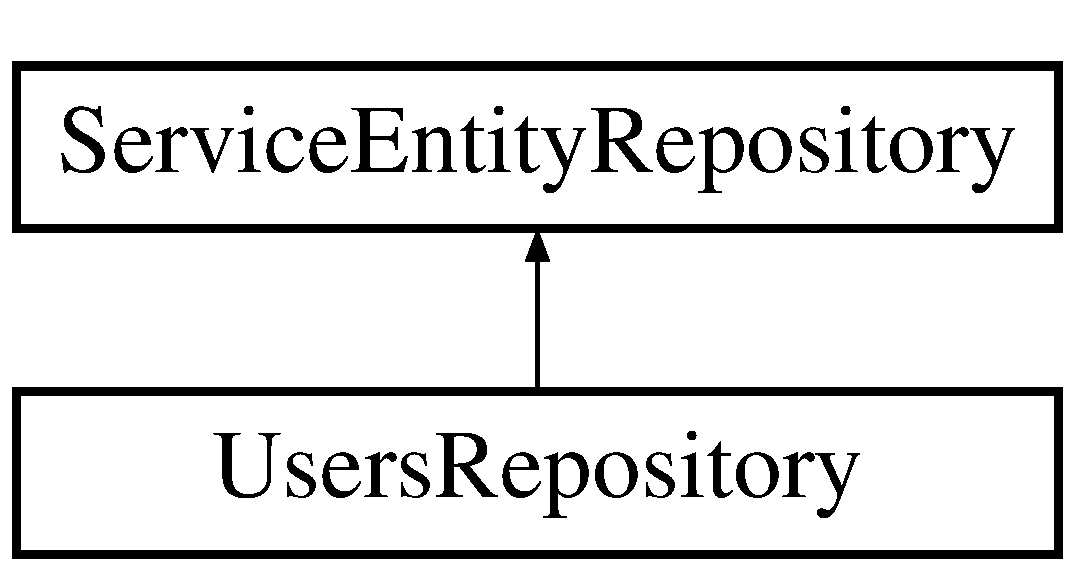
\includegraphics[height=2.000000cm]{class_app_1_1_repository_1_1_users_repository}
\end{center}
\end{figure}
\subsection*{Public Member Functions}
\begin{DoxyCompactItemize}
\item 
\mbox{\hyperlink{class_app_1_1_repository_1_1_users_repository_a38ea33dde11163765f358f5f10a3bc03}{\+\_\+\+\_\+construct}} (Manager\+Registry \$registry)
\end{DoxyCompactItemize}


\subsection{Detailed Description}
Users$\vert$null find(\$id, \$lock\+Mode = null, \$lock\+Version = null)  Users$\vert$null find\+One\+By(array \$criteria, array \$order\+By = null)  Users\mbox{[}\mbox{]} find\+All()  Users\mbox{[}\mbox{]} find\+By(array \$criteria, array \$order\+By = null, \$limit = null, \$offset = null) 

\subsection{Constructor \& Destructor Documentation}
\mbox{\Hypertarget{class_app_1_1_repository_1_1_users_repository_a38ea33dde11163765f358f5f10a3bc03}\label{class_app_1_1_repository_1_1_users_repository_a38ea33dde11163765f358f5f10a3bc03}} 
\index{App\+::\+Repository\+::\+Users\+Repository@{App\+::\+Repository\+::\+Users\+Repository}!\+\_\+\+\_\+construct@{\+\_\+\+\_\+construct}}
\index{\+\_\+\+\_\+construct@{\+\_\+\+\_\+construct}!App\+::\+Repository\+::\+Users\+Repository@{App\+::\+Repository\+::\+Users\+Repository}}
\subsubsection{\texorpdfstring{\+\_\+\+\_\+construct()}{\_\_construct()}}
{\footnotesize\ttfamily \+\_\+\+\_\+construct (\begin{DoxyParamCaption}\item[{Manager\+Registry}]{\$registry }\end{DoxyParamCaption})}



The documentation for this class was generated from the following file\+:\begin{DoxyCompactItemize}
\item 
src/\+Repository/\mbox{\hyperlink{_users_repository_8php}{Users\+Repository.\+php}}\end{DoxyCompactItemize}

\chapter{File Documentation}
\hypertarget{_admin_edit_post_controller_8php}{}\section{src/\+Controller/\+Admin\+Edit\+Post\+Controller.php File Reference}
\label{_admin_edit_post_controller_8php}\index{src/\+Controller/\+Admin\+Edit\+Post\+Controller.\+php@{src/\+Controller/\+Admin\+Edit\+Post\+Controller.\+php}}
\subsection*{Data Structures}
\begin{DoxyCompactItemize}
\item 
class \mbox{\hyperlink{class_app_1_1_controller_1_1_admin_edit_post_controller}{Admin\+Edit\+Post\+Controller}}
\end{DoxyCompactItemize}
\subsection*{Namespaces}
\begin{DoxyCompactItemize}
\item 
 \mbox{\hyperlink{namespace_app_1_1_controller}{App\textbackslash{}\+Controller}}
\end{DoxyCompactItemize}

\hypertarget{_api_shop_controller_8php}{}\section{src/\+Controller/\+Api\+Shop\+Controller.php File Reference}
\label{_api_shop_controller_8php}\index{src/\+Controller/\+Api\+Shop\+Controller.\+php@{src/\+Controller/\+Api\+Shop\+Controller.\+php}}
\subsection*{Data Structures}
\begin{DoxyCompactItemize}
\item 
class \mbox{\hyperlink{class_app_1_1_controller_1_1_api_shop_controller}{Api\+Shop\+Controller}}
\end{DoxyCompactItemize}
\subsection*{Namespaces}
\begin{DoxyCompactItemize}
\item 
 \mbox{\hyperlink{namespace_app_1_1_controller}{App\textbackslash{}\+Controller}}
\end{DoxyCompactItemize}

\hypertarget{_cart_controller_8php}{}\section{src/\+Controller/\+Cart\+Controller.php File Reference}
\label{_cart_controller_8php}\index{src/\+Controller/\+Cart\+Controller.\+php@{src/\+Controller/\+Cart\+Controller.\+php}}
\subsection*{Data Structures}
\begin{DoxyCompactItemize}
\item 
class \mbox{\hyperlink{class_app_1_1_controller_1_1_cart_controller}{Cart\+Controller}}
\end{DoxyCompactItemize}
\subsection*{Namespaces}
\begin{DoxyCompactItemize}
\item 
 \mbox{\hyperlink{namespace_app_1_1_controller}{App\textbackslash{}\+Controller}}
\end{DoxyCompactItemize}

\hypertarget{_mail_contact_controller_8php}{}\section{src/\+Controller/\+Mail\+Contact\+Controller.php File Reference}
\label{_mail_contact_controller_8php}\index{src/\+Controller/\+Mail\+Contact\+Controller.\+php@{src/\+Controller/\+Mail\+Contact\+Controller.\+php}}
\subsection*{Data Structures}
\begin{DoxyCompactItemize}
\item 
class \mbox{\hyperlink{class_app_1_1_controller_1_1_mail_contact_controller}{Mail\+Contact\+Controller}}
\end{DoxyCompactItemize}
\subsection*{Namespaces}
\begin{DoxyCompactItemize}
\item 
 \mbox{\hyperlink{namespace_app_1_1_controller}{App\textbackslash{}\+Controller}}
\end{DoxyCompactItemize}

\hypertarget{_user_controller_8php}{}\section{src/\+Controller/\+User\+Controller.php File Reference}
\label{_user_controller_8php}\index{src/\+Controller/\+User\+Controller.\+php@{src/\+Controller/\+User\+Controller.\+php}}
\subsection*{Data Structures}
\begin{DoxyCompactItemize}
\item 
class \mbox{\hyperlink{class_app_1_1_controller_1_1_user_controller}{User\+Controller}}
\end{DoxyCompactItemize}
\subsection*{Namespaces}
\begin{DoxyCompactItemize}
\item 
 \mbox{\hyperlink{namespace_app_1_1_controller}{App\textbackslash{}\+Controller}}
\end{DoxyCompactItemize}

\hypertarget{_cart_8php}{}\section{src/\+Entity/\+Cart.php File Reference}
\label{_cart_8php}\index{src/\+Entity/\+Cart.\+php@{src/\+Entity/\+Cart.\+php}}
\subsection*{Data Structures}
\begin{DoxyCompactItemize}
\item 
class \mbox{\hyperlink{class_app_1_1_entity_1_1_cart}{Cart}}
\end{DoxyCompactItemize}
\subsection*{Namespaces}
\begin{DoxyCompactItemize}
\item 
 \mbox{\hyperlink{namespace_app_1_1_entity}{App\textbackslash{}\+Entity}}
\end{DoxyCompactItemize}

\hypertarget{_category_8php}{}\section{src/\+Entity/\+Category.php File Reference}
\label{_category_8php}\index{src/\+Entity/\+Category.\+php@{src/\+Entity/\+Category.\+php}}
\subsection*{Data Structures}
\begin{DoxyCompactItemize}
\item 
class \mbox{\hyperlink{class_app_1_1_entity_1_1_category}{Category}}
\end{DoxyCompactItemize}
\subsection*{Namespaces}
\begin{DoxyCompactItemize}
\item 
 \mbox{\hyperlink{namespace_app_1_1_entity}{App\textbackslash{}\+Entity}}
\end{DoxyCompactItemize}

\hypertarget{_commande_8php}{}\section{src/\+Entity/\+Commande.php File Reference}
\label{_commande_8php}\index{src/\+Entity/\+Commande.\+php@{src/\+Entity/\+Commande.\+php}}
\subsection*{Data Structures}
\begin{DoxyCompactItemize}
\item 
class \mbox{\hyperlink{class_app_1_1_entity_1_1_commande}{Commande}}
\end{DoxyCompactItemize}
\subsection*{Namespaces}
\begin{DoxyCompactItemize}
\item 
 \mbox{\hyperlink{namespace_app_1_1_entity}{App\textbackslash{}\+Entity}}
\end{DoxyCompactItemize}

\hypertarget{_produits_8php}{}\section{src/\+Entity/\+Produits.php File Reference}
\label{_produits_8php}\index{src/\+Entity/\+Produits.\+php@{src/\+Entity/\+Produits.\+php}}
\subsection*{Data Structures}
\begin{DoxyCompactItemize}
\item 
class \mbox{\hyperlink{class_app_1_1_entity_1_1_produits}{Produits}}
\end{DoxyCompactItemize}
\subsection*{Namespaces}
\begin{DoxyCompactItemize}
\item 
 \mbox{\hyperlink{namespace_app_1_1_entity}{App\textbackslash{}\+Entity}}
\end{DoxyCompactItemize}

\hypertarget{_role_8php}{}\section{src/\+Entity/\+Role.php File Reference}
\label{_role_8php}\index{src/\+Entity/\+Role.\+php@{src/\+Entity/\+Role.\+php}}
\subsection*{Data Structures}
\begin{DoxyCompactItemize}
\item 
class \mbox{\hyperlink{class_app_1_1_entity_1_1_role}{Role}}
\end{DoxyCompactItemize}
\subsection*{Namespaces}
\begin{DoxyCompactItemize}
\item 
 \mbox{\hyperlink{namespace_app_1_1_entity}{App\textbackslash{}\+Entity}}
\end{DoxyCompactItemize}

\hypertarget{_users_8php}{}\section{src/\+Entity/\+Users.php File Reference}
\label{_users_8php}\index{src/\+Entity/\+Users.\+php@{src/\+Entity/\+Users.\+php}}
\subsection*{Data Structures}
\begin{DoxyCompactItemize}
\item 
class \mbox{\hyperlink{class_app_1_1_entity_1_1_users}{Users}}
\end{DoxyCompactItemize}
\subsection*{Namespaces}
\begin{DoxyCompactItemize}
\item 
 \mbox{\hyperlink{namespace_app_1_1_entity}{App\textbackslash{}\+Entity}}
\end{DoxyCompactItemize}

\hypertarget{_kernel_8php}{}\section{src/\+Kernel.php File Reference}
\label{_kernel_8php}\index{src/\+Kernel.\+php@{src/\+Kernel.\+php}}
\subsection*{Data Structures}
\begin{DoxyCompactItemize}
\item 
class \mbox{\hyperlink{class_app_1_1_kernel}{Kernel}}
\end{DoxyCompactItemize}
\subsection*{Namespaces}
\begin{DoxyCompactItemize}
\item 
 \mbox{\hyperlink{namespace_app}{App}}
\end{DoxyCompactItemize}

\hypertarget{_cart_repository_8php}{}\section{src/\+Repository/\+Cart\+Repository.php File Reference}
\label{_cart_repository_8php}\index{src/\+Repository/\+Cart\+Repository.\+php@{src/\+Repository/\+Cart\+Repository.\+php}}
\subsection*{Data Structures}
\begin{DoxyCompactItemize}
\item 
class \mbox{\hyperlink{class_app_1_1_repository_1_1_cart_repository}{Cart\+Repository}}
\end{DoxyCompactItemize}
\subsection*{Namespaces}
\begin{DoxyCompactItemize}
\item 
 \mbox{\hyperlink{namespace_app_1_1_repository}{App\textbackslash{}\+Repository}}
\end{DoxyCompactItemize}

\hypertarget{_category_repository_8php}{}\section{src/\+Repository/\+Category\+Repository.php File Reference}
\label{_category_repository_8php}\index{src/\+Repository/\+Category\+Repository.\+php@{src/\+Repository/\+Category\+Repository.\+php}}
\subsection*{Data Structures}
\begin{DoxyCompactItemize}
\item 
class \mbox{\hyperlink{class_app_1_1_repository_1_1_category_repository}{Category\+Repository}}
\end{DoxyCompactItemize}
\subsection*{Namespaces}
\begin{DoxyCompactItemize}
\item 
 \mbox{\hyperlink{namespace_app_1_1_repository}{App\textbackslash{}\+Repository}}
\end{DoxyCompactItemize}

\hypertarget{_commande_repository_8php}{}\section{src/\+Repository/\+Commande\+Repository.php File Reference}
\label{_commande_repository_8php}\index{src/\+Repository/\+Commande\+Repository.\+php@{src/\+Repository/\+Commande\+Repository.\+php}}
\subsection*{Data Structures}
\begin{DoxyCompactItemize}
\item 
class \mbox{\hyperlink{class_app_1_1_repository_1_1_commande_repository}{Commande\+Repository}}
\end{DoxyCompactItemize}
\subsection*{Namespaces}
\begin{DoxyCompactItemize}
\item 
 \mbox{\hyperlink{namespace_app_1_1_repository}{App\textbackslash{}\+Repository}}
\end{DoxyCompactItemize}

\hypertarget{_produits_repository_8php}{}\section{src/\+Repository/\+Produits\+Repository.php File Reference}
\label{_produits_repository_8php}\index{src/\+Repository/\+Produits\+Repository.\+php@{src/\+Repository/\+Produits\+Repository.\+php}}
\subsection*{Data Structures}
\begin{DoxyCompactItemize}
\item 
class \mbox{\hyperlink{class_app_1_1_repository_1_1_produits_repository}{Produits\+Repository}}
\end{DoxyCompactItemize}
\subsection*{Namespaces}
\begin{DoxyCompactItemize}
\item 
 \mbox{\hyperlink{namespace_app_1_1_repository}{App\textbackslash{}\+Repository}}
\end{DoxyCompactItemize}

\hypertarget{_role_repository_8php}{}\section{src/\+Repository/\+Role\+Repository.php File Reference}
\label{_role_repository_8php}\index{src/\+Repository/\+Role\+Repository.\+php@{src/\+Repository/\+Role\+Repository.\+php}}
\subsection*{Data Structures}
\begin{DoxyCompactItemize}
\item 
class \mbox{\hyperlink{class_app_1_1_repository_1_1_role_repository}{Role\+Repository}}
\end{DoxyCompactItemize}
\subsection*{Namespaces}
\begin{DoxyCompactItemize}
\item 
 \mbox{\hyperlink{namespace_app_1_1_repository}{App\textbackslash{}\+Repository}}
\end{DoxyCompactItemize}

\hypertarget{_users_repository_8php}{}\section{src/\+Repository/\+Users\+Repository.php File Reference}
\label{_users_repository_8php}\index{src/\+Repository/\+Users\+Repository.\+php@{src/\+Repository/\+Users\+Repository.\+php}}
\subsection*{Data Structures}
\begin{DoxyCompactItemize}
\item 
class \mbox{\hyperlink{class_app_1_1_repository_1_1_users_repository}{Users\+Repository}}
\end{DoxyCompactItemize}
\subsection*{Namespaces}
\begin{DoxyCompactItemize}
\item 
 \mbox{\hyperlink{namespace_app_1_1_repository}{App\textbackslash{}\+Repository}}
\end{DoxyCompactItemize}

%--- End generated contents ---

% Index
\backmatter
\newpage
\phantomsection
\clearemptydoublepage
\addcontentsline{toc}{chapter}{Index}
\printindex

\end{document}
